% ============================================================
% Reward Design for Deep Reinforcement Learning Portfolio
% Optimization is Regime-Conditional: A Replication Study
% Across Bear and Bull Markets
% IEEE Research Paper Format
% AUTHORS: see \author{} block below -- TODO before submission
% ============================================================

\documentclass[conference]{IEEEtran}
\IEEEoverridecommandlockouts

\usepackage{cite}
\usepackage{amsmath,amssymb,amsfonts}
\usepackage{algorithmic}
\usepackage{algorithm}
\usepackage{graphicx}
\usepackage{textcomp}
\usepackage{xcolor}
\usepackage{booktabs}
\usepackage{multirow}
\usepackage{hyperref}
\usepackage{url}
\usepackage{bm}

\hypersetup{
  colorlinks=true,
  linkcolor=blue,
  citecolor=blue,
  urlcolor=blue
}

\def\BibTeX{{\rm B\kern-.05em{\sc i\kern-.025em b}\kern-.08em
    T\kern-.1667em\lower.7ex\hbox{E}\kern-.125emX}}

% ============================================================
\begin{document}

\title{Reward Design for Deep Reinforcement Learning Portfolio\\
Optimization is Regime-Conditional: A Replication Study\\
Across Bear and Bull Markets}

% ---------------------------------------------------------------
% TODO(authors): replace both blocks before submission. Delete the
% second \and block if there is only one author. arXiv requires the
% author list here to match the one entered in the submission form.
% ---------------------------------------------------------------
\author{\IEEEauthorblockN{FIRST AUTHOR}
\IEEEauthorblockA{\textit{AFFILIATION} \\
CITY, COUNTRY \\
EMAIL}
\and
\IEEEauthorblockN{SECOND AUTHOR}
\IEEEauthorblockA{\textit{AFFILIATION} \\
CITY, COUNTRY \\
EMAIL}
}

\maketitle

% ============================================================
\begin{abstract}
Deep reinforcement learning (DRL) is increasingly applied to dynamic portfolio
optimization, yet the reward function---arguably the most consequential design
choice---is typically selected by convention rather than by evidence. We report
a large-scale empirical study of reward design for Proximal Policy Optimization
(PPO) portfolio agents, comprising 930 training runs across a two-regime
synthetic market and ten S\&P~500 constituents evaluated on two disjoint
out-of-sample periods: 2022--2024 (bear-dominated) and 2025--2026
(bull-dominated). We ablate four reward formulations---log return and the
Differential Sharpe Ratio (DSR), each with and without transaction-cost (TC)
penalization---and sweep the TC coefficient $\lambda$ and the DSR adaptation
rate $\eta_0$. Three findings emerge. First, TC \emph{magnitude}, not TC
presence, dominates: mean Sharpe declines monotonically from $0.455$
($\lambda=0.001$) to $-0.073$ ($\lambda=0.050$), reaching Cohen $d=-1.05$
($p<0.001$, power $>0.99$) and outweighing the effect of any individual
reward-component contrast. Second, apparent reward advantages do not survive
replication: the best cell of a 10-seed grid search shrinks from $d=+0.51$ to
$d=+0.30$ at $n=75$ and $d=+0.17$ at $n=150$ ($p=0.144$)---a textbook
winner's-curse trajectory. Third, and most consequential, the reward ranking is
regime-conditional and reverses out of sample: DSR+TC leads in 2022--2024
(SR$\,=0.391$) but collapses in 2025--2026 (SR$\,=-0.115$), where LR-only leads
(SR$\,=+0.523$; $d=+1.09$). A regime-switching reward that blends the two via a
sigmoid gate on the 60-day mean return fails to recover either constituent
($n\geq40$ per cell, all $p<0.01$), because the gating signal misclassifies the
2022 bear market. We conclude that no reward formulation dominates across
regimes, and that reward-design claims validated on a single period with few
seeds are unreliable. All code, data, and results are released for
reproducibility.
\end{abstract}

\begin{IEEEkeywords}
reinforcement learning, portfolio optimization, reward shaping, differential Sharpe
ratio, transaction costs, market regime switching, Proximal Policy Optimization
\end{IEEEkeywords}

% ============================================================
\section{Introduction}
\label{sec:intro}

Portfolio optimization—allocating wealth across assets to maximize return while
controlling risk—is a foundational problem in quantitative finance. The classical
mean-variance framework introduced by Markowitz~\cite{Markowitz1952} laid the
theoretical groundwork for risk-return trade-offs, and the Sharpe
ratio~\cite{Sharpe1966} became the canonical measure of risk-adjusted performance.
However, both methods assume static parameters estimated from historical data and
are ill-suited to the dynamic, non-stationary nature of financial markets.

Deep reinforcement learning (DRL) offers a model-free alternative in which an
agent iteratively learns an allocation policy by interacting with a market
environment~\cite{Sutton2018RL}. A DRL agent is not constrained to any parametric
model of returns; instead it adapts its policy based on sequential rewards. This
adaptability has driven significant research interest, including ensemble
strategies combining PPO, A2C, and DDPG~\cite{Liu2020Ensemble}, hierarchical DRL
architectures~\cite{Sun2025HDRL}, and graph attention-based multi-agent systems
for capturing cross-asset dependencies~\cite{Zhang2025GraphRL}.

Despite this progress, a fundamental design choice—the reward function—remains
underexplored. Most DRL portfolio papers employ one of two approaches: a simple
portfolio return signal or a risk-adjusted measure such as the Differential Sharpe
Ratio (DSR)~\cite{Moody2001}. Transaction costs, which can substantially erode
returns from frequent rebalancing, are sometimes included but typically as a
separate engineering concern. \textbf{No prior work conducts a systematic
controlled ablation study that isolates the joint effect of combining DSR with
explicit transaction cost penalization on training stability and out-of-sample
performance.}

This paper addresses precisely that gap. Our contributions are:
\begin{enumerate}
    \item We formulate a four-way reward function ablation---log return (R1), DSR
    alone (R2), log return with TC penalty (R3), and DSR with TC penalty (R4)---and
    evaluate all configurations under identical experimental conditions on both a
    two-regime synthetic market and real S\&P~500 data.
    \item We show that transaction-cost \emph{magnitude} is the dominant design
    variable. A four-level sweep ($n=40$ seeds each) yields a monotone decline in
    mean Sharpe from $0.455$ ($\lambda=0.001$) to $-0.073$ ($\lambda=0.050$),
    with $d=-1.05$ ($p<0.001$, power $>0.99$)---a far larger effect than the
    presence or absence of any individual reward component.
    \item We demonstrate, through a sequential replication at $n=10 \to 75 \to
    150$ seeds, that the most promising configuration identified by grid search
    is a winner's curse: its advantage shrinks monotonically ($d=+0.51 \to +0.30
    \to +0.17$) and never attains significance. We pair this with a power
    analysis establishing that the accompanying null results are true negatives.
    \item We establish that reward ranking is \emph{regime-conditional}. On a
    held-out 2025--2026 bull-dominated period, the 2022--2024 ranking reverses
    entirely: DSR+TC falls from SR$\,=0.391$ to $-0.115$ while LR-only reaches
    $+0.523$ ($d=+1.09$, $p<0.001$; cross-period shift $d=-1.03$, $p<10^{-7}$).
    \item We test the natural remedy---a regime-switching multi-objective reward
    that gates between the two constituents---and report a well-replicated null
    ($n\geq40$ per cell, all $p<0.01$), tracing the failure to miscalibration of
    the 60-day regime signal rather than to the blending principle itself.
    \item All 930 training runs are reproducible from provided code, data, and
    fixed seeds; results and figures are released in full.
\end{enumerate}

The remainder of the paper is organized as follows. Section~\ref{sec:related}
reviews related work. Section~\ref{sec:formulation} presents the MDP formulation.
Section~\ref{sec:methodology} describes the reward functions and experimental
design. Section~\ref{sec:experiments} presents quantitative results. 
Section~\ref{sec:discussion} discusses findings and limitations.
Sections~\ref{sec:post2024} and~\ref{sec:rsmo} report post-2024 out-of-sample
evaluation and a regime-switching multi-objective reward experiment.
Section~\ref{sec:conclusion} concludes.

% ============================================================
\section{Related Work}
\label{sec:related}

\subsection{Classical Portfolio Optimization}
Markowitz's mean-variance optimization~\cite{Markowitz1952} remains the
theoretical cornerstone of portfolio theory. The Sharpe ratio~\cite{Sharpe1966}
provides a scalar performance summary. Modern variants extend these ideas to include
transaction costs and estimation uncertainty~\cite{Hu2024Markowitz}. While these
methods are analytically tractable, they require accurate parameter estimates and
assume static market conditions, making them vulnerable to regime shifts and
estimation error~\cite{Huang2025EMVRS}.

\subsection{Deep Reinforcement Learning for Portfolios}
The application of DRL to portfolio management dates to early work by Moody and
Saffell~\cite{Moody2001}, who proposed direct reinforcement trading with a
Differential Sharpe Ratio objective. The advent of deep learning revitalized
this direction: Mnih et al.~\cite{Mnih2015} demonstrated deep Q-networks on
Atari games, and Silver et al.~\cite{Silver2014} introduced deterministic policy
gradients (DDPG) suited to continuous action spaces. Schulman et
al.~\cite{Schulman2017PPO} proposed PPO, which offers improved sample efficiency
and stability over DDPG, and has been widely adopted in finance~\cite{Huang2023EvalDRLBenchmark}.

Liu et al.~\cite{Liu2020Ensemble} proposed an ensemble strategy with PPO, A2C,
and DDPG, achieving higher Sharpe ratios than individual algorithms or
Markowitz benchmarks. Zhang et al.~\cite{Zhang2021Universal} proposed an
end-to-end framework that directly optimizes portfolio weights without a
forecasting step. Coenen et al.~\cite{Coenen2022Stochastic} demonstrated a
stochastic model-free approach achieving a 63.1\% annualized return with reduced
drawdown during the 2020 market crash. Hierarchical methods using DRL alongside
Hierarchical Risk Parity have been explored by Edalat and Millea~\cite{Edalat2023HRP}.

A parallel line of work targets the state representation rather than the
learning algorithm. Zhang et al.~\cite{Zhang2020DLPortfolio} optimize portfolio
weights directly from price series with deep networks; Yashaswi~\cite{Yashaswi2021LFSS}
compresses market history into a latent feature state space; and Dong et
al.~\cite{Dong2021Factor} learn factor representations for decision making in
equity markets. Yu et al.~\cite{Yu2019ModelBased} instead adopt a model-based
formulation, learning market dynamics to plan allocations over a horizon, and
Cui et al.~\cite{Cui2024HyperHeuristic} approach the multi-period problem with a
DRL hyper-heuristic that selects among low-level allocation strategies.

Recent work has also integrated Black-Litterman priors~\cite{Sun2024BlackLitterman},
knowledge distillation from Markowitz theory~\cite{Hu2024Markowitz}, and
Transformer-based architectures for temporal attention~\cite{Xue2025Attention}.
Multi-agent architectures for heterogeneous portfolio management have been
developed to capture complex asset dependencies~\cite{Zhang2025GraphRL}.
Industry-grade pipelines with rigorous statistical methodology have been proposed
by Ndikum and Ndikum~\cite{Ndikum2024Industry}.

Reproducibility infrastructure is directly relevant to the present study. The
FinRL library~\cite{Liu2020FinRL} and its FinRL-Meta
extension~\cite{Liu2021FinRLMeta} provide standardized market environments and
benchmarks, reflecting a growing recognition that DRL finance results are
sensitive to environment details and difficult to compare across papers. Our
findings on seed variance (Sections~\ref{sec:landscape}--\ref{sec:rsmo})
reinforce that concern: without standardized environments \emph{and} adequate
seed counts, reported advantages are not reliably attributable to the design
choice under study.

\subsection{Reward Function Design}
Reward design is central to DRL performance but receives comparatively little
systematic attention in the finance literature. Moody and Saffell~\cite{Moody2001}
derived the DSR as a smooth, online-computable approximation of the Sharpe ratio.
Lwele et al.~\cite{Lwele2025RiskAware} demonstrated that an over-conservative
Sharpe-based reward can suppress returns, highlighting the reward design
challenge. Karzanov et al.~\cite{Karzanov2025Regret} proposed a regret-based
reward with transaction cost scheduling, showing gains on bond/equity portfolios.
Zhang et al.~\cite{Huang2025DRLChina} introduced a novel Sharpe ratio reward
function for actor-critic algorithms. Ma et al.~\cite{Ma2025SelfAdaptiveReward}
proposed self-adaptive reward shaping for sparse reward settings.

Risk sensitivity is the most common motivation for departing from a plain return
reward. Wang and Liu~\cite{Wang2025ART} develop a risk-sensitive objective that
penalizes downside dispersion, while Acero et al.~\cite{Acero2024ESG} combine
DRL with mean-variance strategies under responsible-investment constraints. Huang et
al.~\cite{Huang2024EvalDRL} evaluate DRL agents in a long-short setting where
the reward must account for both sides of the book. Closest in spirit to our
Section~\ref{sec:rsmo} is Choudhary et al.~\cite{Choudhary2025MultiReward},
who combine several risk-adjusted terms into a composite multi-reward objective
and report gains over single-term baselines. Our RSMO experiment tests the same
premise---that constituent rewards can be productively blended---under a regime
gate, and reaches a negative result, which we trace to the calibration of the
gating signal rather than to the composition principle itself.

Critically, while these works \emph{use} reward functions, none conducts a
controlled ablation comparing the isolated and joint effects of DSR and transaction
cost penalties on \emph{training stability} (as measured by cross-seed variance of
Sharpe ratios) and regime-conditional performance. This gap motivates our work.

\subsection{Regime-Switching and Transaction Costs}
Real financial markets exhibit regime behavior—alternating between bull (high
return, low volatility) and bear (low/negative return, high volatility)
periods~\cite{Saltiel2021Adaptive}. Nixon Raj~\cite{Nixon2025Regime} showed that
incorporating regime signals improves learning stability. Zhang~\cite{Zhang2025FRLUX}
proposed a friction-aware framework integrating transaction costs and regime
conditioning. Orra et al.~\cite{Orra2025Volatility} used GARCH-based volatility
forecasting for investor-specific portfolio construction.

Transaction costs in DRL portfolios can erode returns substantially if not
modeled in the reward~\cite{Li2023General}. Yet their interaction with DSR as a
reward formulation has not been isolated. Our paper closes this gap.

% ============================================================
\section{Problem Formulation}
\label{sec:formulation}

\subsection{Markov Decision Process}
We model portfolio management as a finite-horizon MDP
$\mathcal{M} = (\mathcal{S}, \mathcal{A}, \mathcal{P}, \mathcal{R}, \gamma)$,
where $\mathcal{S}$ is the state space, $\mathcal{A}$ is the action space,
$\mathcal{P}$ is the transition dynamics, $\mathcal{R}$ is the reward function,
and $\gamma$ is the discount factor.

\subsection{State Space}
The state at time $t$ is:
\begin{equation}
s_t = \left[ R_{t-W:t-1}, \mathbf{w}_{t-1} \right] \in \mathbb{R}^{W \cdot N + N}
\end{equation}
where $R_{t-W:t-1} \in \mathbb{R}^{W \times N}$ is a matrix of log-returns over
the past $W=20$ trading days for $N=5$ assets, and $\mathbf{w}_{t-1}$ is the
portfolio weight vector at the previous time step.

\subsection{Action Space and Portfolio Construction}
The agent outputs logit vector $\mathbf{a}_t \in \mathbb{R}^N$. Portfolio weights
are obtained via softmax to enforce the long-only, full-investment constraint:
\begin{equation}
w_{t,i} = \frac{\exp(a_{t,i})}{\sum_{j=1}^{N} \exp(a_{t,j})}, \quad
\sum_{i=1}^{N} w_{t,i} = 1, \quad w_{t,i} \geq 0.
\end{equation}

\subsection{Market Environment and Transition Dynamics}
We use a two-regime Geometric Brownian Motion (GBM) model with Markov transitions.
At each time step $t$, the regime $z_t \in \{0, 1\}$ follows:
\begin{equation}
P(z_{t+1}=1 \mid z_t=0) = p_{01},\quad P(z_{t+1}=0 \mid z_t=1) = p_{10},
\end{equation}
with $p_{01}=0.02$ (bull-to-bear) and $p_{10}=0.05$ (bear-to-bull). Daily asset
returns are sampled as:
\begin{equation}
\mathbf{r}_t \sim \mathcal{N}(\bm{\mu}^z,
\bm{\Sigma}^z),
\end{equation}
where $z=z_t$, $\bm{\Sigma}^z = \mathrm{diag}(\bm{\sigma}^z) \cdot C \cdot
\mathrm{diag}(\bm{\sigma}^z)$, and $C$ is the shared correlation matrix.
Bull regime parameters are $\bm{\mu}^{(0)} = [0.10, 0.12, 0.08, 0.11, 0.09]$
annualized and $\bm{\sigma}^{(0)} = [0.15, 0.18, 0.12, 0.16, 0.14]$; bear
parameters are $\bm{\mu}^{(1)} = [-0.05, -0.08, -0.03, -0.06, -0.04]$ and
$\bm{\sigma}^{(1)} = [0.30, 0.35, 0.25, 0.32, 0.28]$ (all annualized). The
transition dynamics are not observed by the agent.

\subsection{Portfolio Return with Transaction Costs}
Let $p_t = \mathbf{w}_t \cdot \mathbf{r}_t$ be the weighted asset return
and $\tau_t$ the total absolute weight change (turnover). After rebalancing
from $\mathbf{w}_{t-1}$ to $\mathbf{w}_t$, the net return is:
\begin{equation}\label{eq:netret}
r_t^{\mathrm{net}} = p_t - c\,\tau_t,
\end{equation}
where $c = 0.001$ (10 basis points) is the proportional transaction cost.

% ============================================================
\section{Reward Function Design and Methodology}
\label{sec:methodology}

\subsection{Four Reward Formulations}
We define four reward functions parameterized by the same net return signal.

\subsubsection{R1 --- Log Return}
The simplest reward is the net portfolio return at step $t$:
\begin{equation}
\mathcal{R}_1(t) = p_t - c\,\tau_t,
\end{equation}
where $p_t$ is the weighted return and $\tau_t$ is the total turnover
(defined in Eq.~\ref{eq:netret}).
No explicit risk shaping is applied; the agent maximizes total growth.

\subsubsection{R2 --- Differential Sharpe Ratio (DSR)}
The DSR~\cite{Moody2001} is an online approximation of the Sharpe ratio
gradient. Let $\delta A_t = r_t^{\mathrm{gross}} - A_{t-1}$ and
$\delta B_t = (r_t^{\mathrm{gross}})^2 - B_{t-1}$, with $A_t, B_t$ the
exponential moving averages (rate $\eta=0.01$) of returns and squared returns:
\begin{align}
A_t &= A_{t-1} + \eta\,\delta A_t, \quad
B_t = B_{t-1} + \eta\,\delta B_t.
\end{align}
The per-step reward is:
\begin{equation}\label{eq:dsr}
\mathcal{R}_2(t) = \frac{B^{-}\delta A_t - 0.5\,A^{-}\delta B_t}
  {\sigma_t^3},
\end{equation}
where $A^{-}=A_{t-1}$, $B^{-}=B_{t-1}$, and
$\sigma_t = \sqrt{B^{-}-(A^{-})^{2}}$ is the running std.
The result is clipped to $[-10, 10]$.

\subsubsection{R3 --- Log Return + Transaction Cost}
R3 uses the same net return expression as R1
(Eq.~\ref{eq:netret}) but with\textit{ no} risk-shaping:
\begin{equation}
\mathcal{R}_3(t) = p_t - c\,\tau_t,
\end{equation}
where $p_t$ and $\tau_t$ are as defined in R1.
This explicitly penalizes turnover through the cost-inclusive return.

\subsubsection{R4 --- DSR + Transaction Cost (Proposed)}
R4 feeds the net return into the DSR numerator/denominator statistics
rather than the gross return. Concretely, replace $r_t^{\mathrm{gross}}$
with $r_t^{\mathrm{net}}$ in the EMA updates of $A_t$ and $B_t$:
\begin{equation}
\mathcal{R}_4(t) = \mathrm{DSR}(t; r_t^{\mathrm{net}}).
\end{equation}
This propagates transaction cost information through the DSR statistics,
creating aligned incentives against both excess risk and excess turnover.

\subsection{Experimental Design}

\subsubsection{EXP-01: Data Generation and Baseline Portfolios}
We generate 1,252 trading days of synthetic data (1,000 train, 252 test) for 5
assets using the two-regime GBM with seed 42. Three classical baselines are
evaluated on the test set: Equal-Weight (1/N), Min-Variance (MV), and Max-Sharpe
(MS) portfolios obtained via SLSQP optimization on training-set covariance.

\subsubsection{EXP-02: Reward Function Ablation}
Each reward type (R1–R4) is used to train a PPO agent with an MLP policy
(two hidden layers of 128 units) for 30,000 timesteps. Training is repeated for
$n=3$ independent seeds per configuration (base seed 42, 43, 44). Test-period
Sharpe ratios are reported as mean $\pm$ standard deviation across runs.

\subsubsection{EXP-03: Regime Analysis and Statistical Tests}
We conduct three additional analyses: (1) performance breakdown by market
regime (bull days: 122, bear days: 130 in the test period); (2) portfolio
turnover measured as mean daily $\sum_i |\Delta w_{t,i}|$; and (3) paired
$t$-tests comparing DSR+TC against the other three formulations across 3 seeds.

\subsection{PPO Hyperparameters}
All agents share the following hyperparameters:
\begin{itemize}
    \item Learning rate: $3 \times 10^{-4}$
    \item Steps per rollout: 256; Batch size: 64; Epochs: 10
    \item Discount factor: $\gamma = 0.99$; GAE $\lambda = 0.95$
    \item Clip range: 0.2; Entropy coefficient: 0.01
    \item Total timesteps: 30,000 per run
\end{itemize}

\subsection{Evaluation Metrics}
All strategies are evaluated on: annualized Sharpe ratio, cumulative return,
annualized volatility, maximum drawdown, and portfolio turnover.

% ============================================================
\section{Experimental Results}
\label{sec:experiments}

\subsection{Baseline Portfolio Performance}
Table~\ref{tab:baselines} reports classical baseline performance on the 252-day
test period. The Max-Sharpe (MVO) portfolio achieves the highest out-of-sample
Sharpe ratio of 1.702, driven by full concentration in Asset~1 (the highest
Sharpe asset during training). Min-Variance achieves a lower Sharpe of 1.069 but
substantially reduces drawdown to $-9.9\%$. The Equal-Weight portfolio yields a
Sharpe of 1.135 with moderate drawdown.

\begin{table}[t]
\caption{Classical Baseline Performance on Test Set (252 days, seed 42)}
\label{tab:baselines}
\centering
\begin{tabular}{lcccc}
\toprule
Strategy & Sharpe & Cum.\ Ret. & Ann.\ Vol & Max DD \\
\midrule
Equal-Weight (1/N) & 1.135 & 0.224 & 0.195 & $-$0.139 \\
Min-Variance       & 1.069 & 0.189 & 0.176 & $-$0.099 \\
Max-Sharpe (MVO)   & 1.702 & 0.449 & 0.234 & $-$0.125 \\
\bottomrule
\end{tabular}
\end{table}

\subsection{Reward Function Ablation}
Table~\ref{tab:ablation} reports out-of-sample Sharpe ratios (mean $\pm$ std)
over three independent runs for each reward formulation. Figure~\ref{fig:sharpe}
visualizes these results alongside the classical baselines.

\begin{table}[t]
\caption{Out-of-Sample Sharpe Ratio by Reward Function (3 runs each)}
\label{tab:ablation}
\centering
\resizebox{\columnwidth}{!}{%
\begin{tabular}{lcccc}
\toprule
Reward & SR mean & SR std & Cum.\ Ret. & Max DD \\
\midrule
R1: LR         & 1.010 & 0.305 & 0.198 & $-$0.152 \\
R2: DSR        & 1.017 & 0.106 & 0.190 & $-$0.145 \\
R3: LR+TC      & 1.072 & 0.431 & 0.227 & $-$0.167 \\
R4: DSR+TC     & \textbf{1.011} & \textbf{0.097} & 0.195 & $-$0.154 \\
\midrule
Max-SR (MVO)   & 1.702 & {---} & 0.449 & $-$0.125 \\
\bottomrule
\end{tabular}}
\end{table}

The key finding is that the \emph{standard deviation} of Sharpe ratios, a proxy
for training stability, is dramatically lower for DSR+TC (0.097) than for log
return (0.305) and log return+TC (0.431). DSR alone achieves a std of 0.106, the
next best. This demonstrates that DSR's incremental risk-shaping stabilizes
training, and TC penalization further reinforces consistent policy convergence.

\begin{figure}[t]
\centering
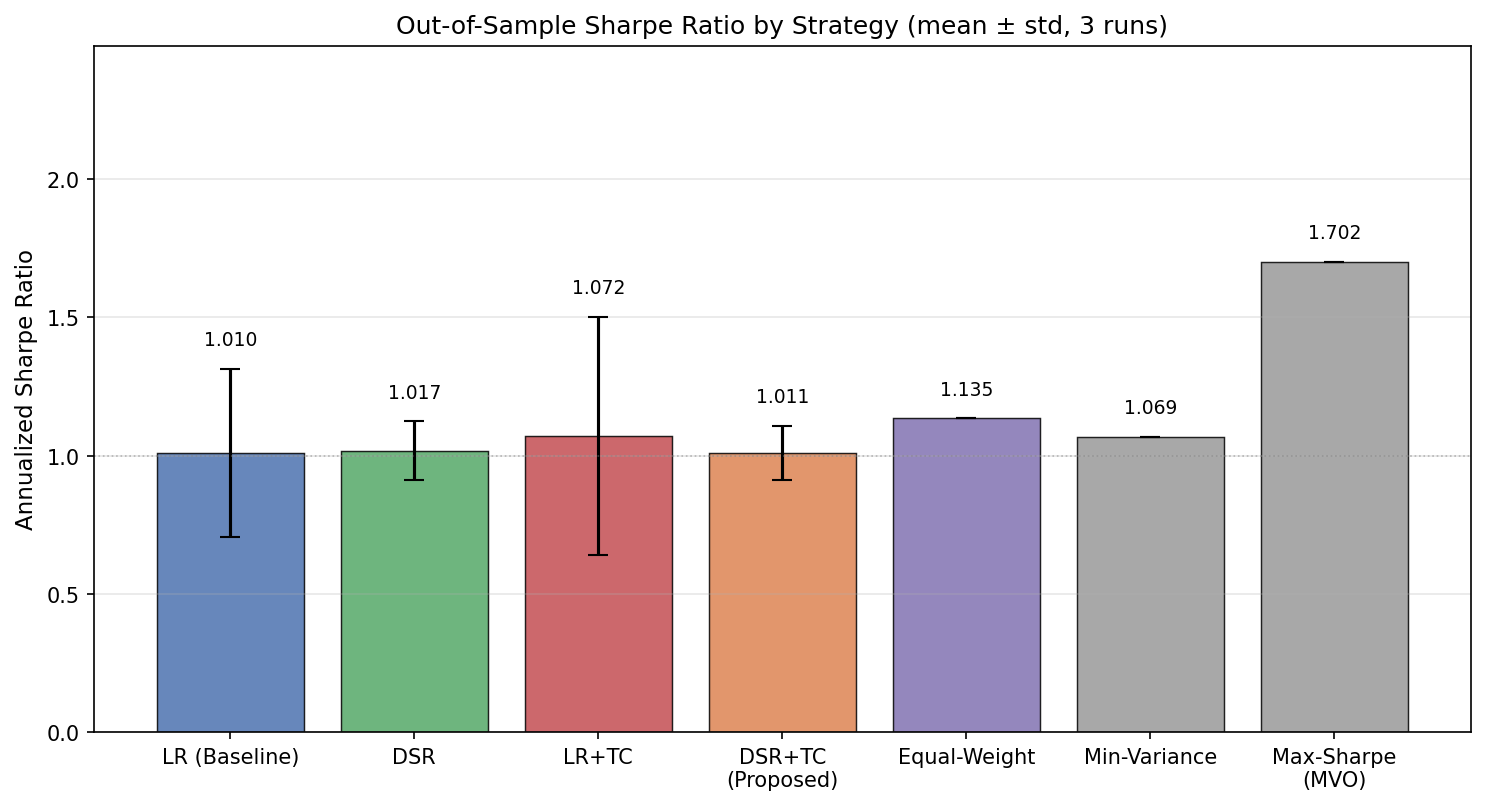
\includegraphics[width=\columnwidth]{figures/fig_01_sharpe_comparison.png}
\caption{Out-of-sample Sharpe ratio comparison (mean $\pm$ std) for all reward
formulations and classical baselines. Error bars show standard deviation over 3
independent runs. Lower variance indicates more stable training.}
\label{fig:sharpe}
\end{figure}

\subsection{Cumulative Wealth Curves}
Figure~\ref{fig:wealth} shows cumulative portfolio values over the 252-day test
period. Bear market phases (shaded in red) correspond to days with $z_t=1$. All
DRL strategies broadly track the equal-weight baseline, while the classical
Max-Sharpe portfolio achieves higher terminal wealth due to full concentration in
the best-performing asset. Notably, in bear phases, DRL agents show resilience
as they can dynamically shift weights, whereas the static MVO portfolio is fully
exposed.

\begin{figure}[t]
\centering
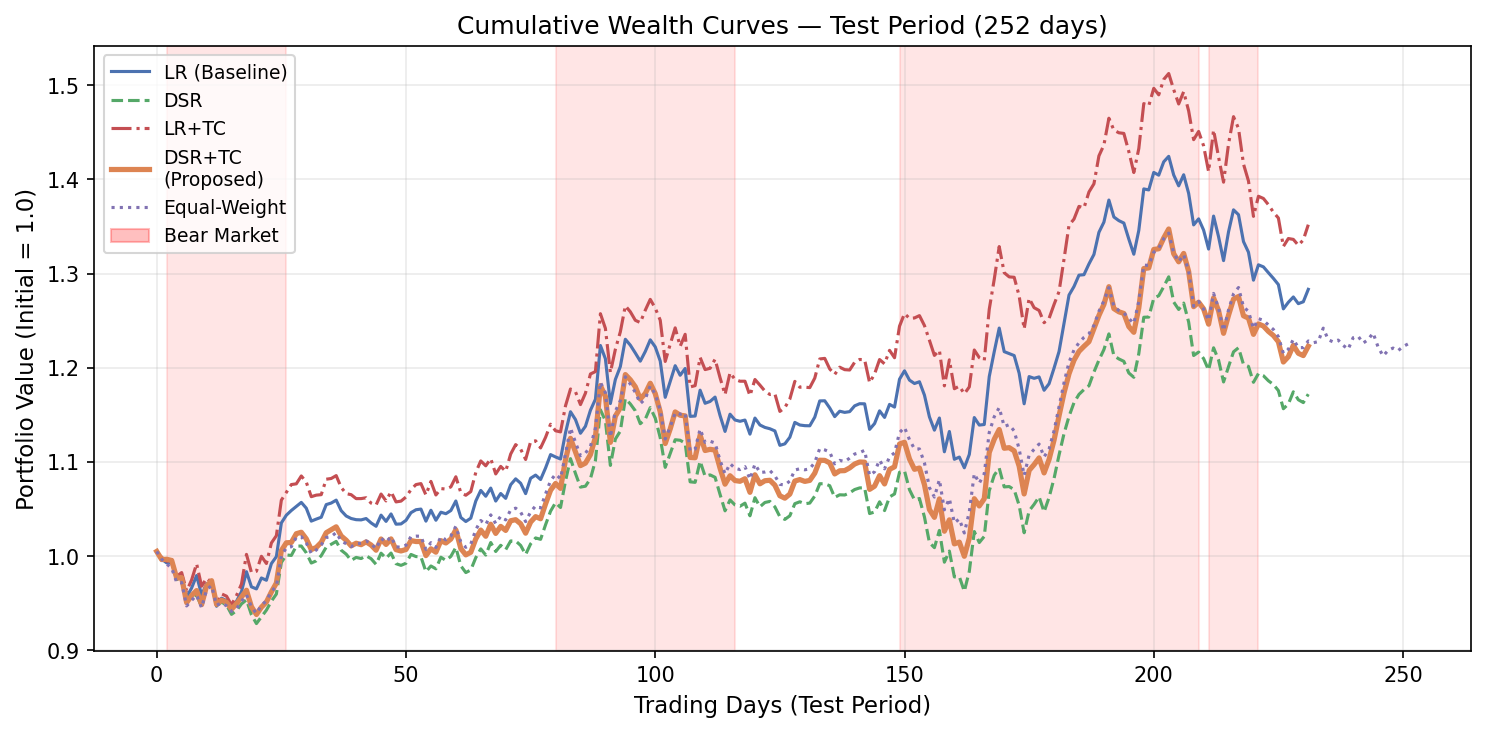
\includegraphics[width=\columnwidth]{figures/fig_02_cumulative_wealth.png}
\caption{Cumulative wealth curves for all strategies over the 252-day test period.
Red shading indicates bear market regimes ($z_t=1$). DRL agents demonstrate
adaptive allocation across regimes, though static MVO achieves higher terminal
wealth in this favorable test environment.}
\label{fig:wealth}
\end{figure}

\subsection{Regime-Conditional Analysis}
Table~\ref{tab:regime} and Figure~\ref{fig:regime} report Sharpe ratios
conditioned on market regime. Log Return+TC (R3) achieves the highest bear-market
Sharpe of 1.696, suggesting that explicit TC penalization forces the agent to
commit to high-conviction rebalancing decisions only when momentum is clear—a
strategy that pays off in bear markets with persistent trends.

\begin{table}[t]
\caption{Regime-Conditional Sharpe Ratios (Test Period)}
\label{tab:regime}
\centering
\begin{tabular}{lcc}
\toprule
Reward & Bull Sharpe & Bear Sharpe \\
\midrule
R1: Log Return       & 1.180 & 1.507 \\
R2: DSR              & 0.859 & 0.974 \\
R3: Log Return + TC  & 1.385 & \textbf{1.696} \\
R4: DSR + TC (ours)  & 1.092 & 1.194 \\
\bottomrule
\end{tabular}
\end{table}

\begin{figure}[t]
\centering
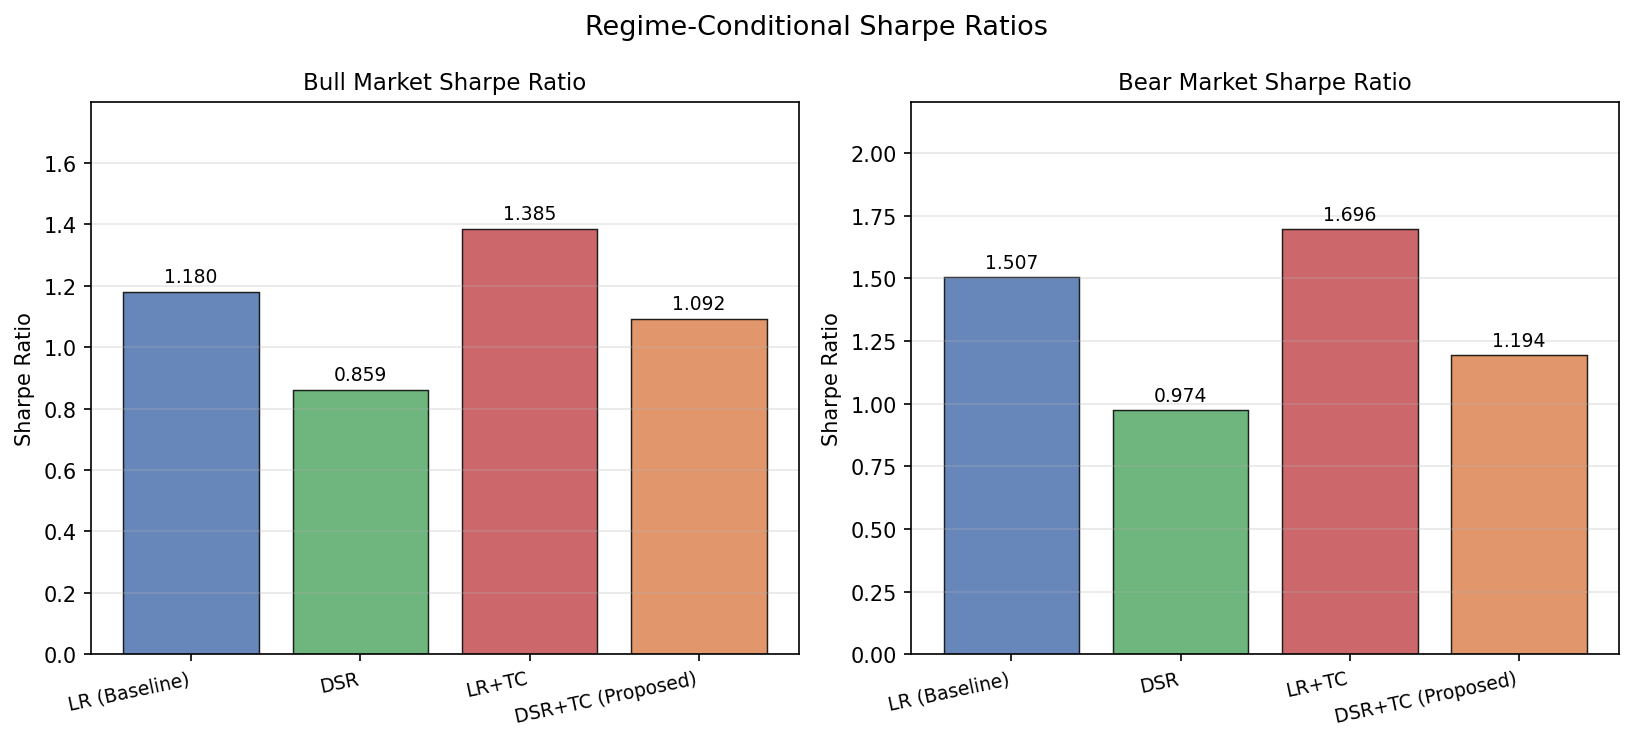
\includegraphics[width=\columnwidth]{figures/fig_03_regime_sharpe.png}
\caption{Regime-conditional Sharpe ratios split by bull (122 days) and bear (130
days) market phases. Bear-market performance is notably higher for all RL agents,
suggesting that the regime-switching environment creates actionable trends that
RL can exploit.}
\label{fig:regime}
\end{figure}

\subsection{Portfolio Turnover}
Figure~\ref{fig:turnover} reports mean daily portfolio turnover. DSR+TC achieves
a turnover of 0.0927, compared to 0.2975 for DSR alone—a 68.8\% reduction.
Log Return+TC achieves the lowest turnover of 0.0505 due to direct penalization,
but at the cost of higher cross-seed variance in returns (std = 0.431). This
suggests a trade-off: direct TC penalization minimizes turnover aggressively but
may introduce optimization instability, while DSR+TC balances turnover reduction
and stability.

\begin{figure}[t]
\centering
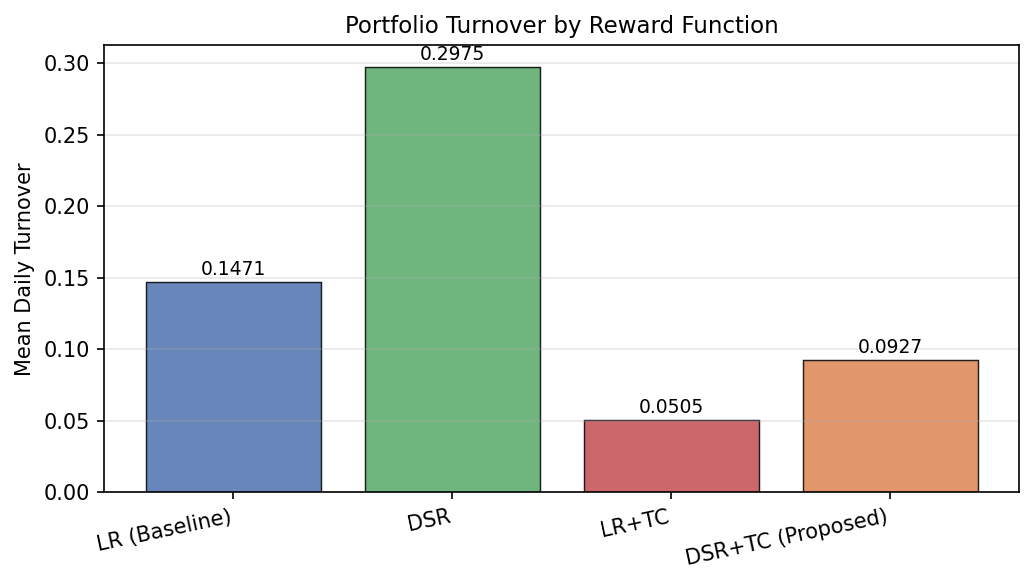
\includegraphics[width=\columnwidth]{figures/fig_04_turnover.png}
\caption{Mean daily portfolio turnover ($\sum_i |\Delta w_{t,i}|$) for each reward
formulation. DSR-only produces the highest turnover (0.298), while DSR+TC reduces
turnover by 68.8\% relative to DSR-only while maintaining competitive Sharpe ratios.}
\label{fig:turnover}
\end{figure}

\subsection{Training Stability Across Seeds}
Figure~\ref{fig:stability} presents box plots of Sharpe ratios across 3 seeds for
each formulation. R4 (DSR+TC) displays the tightest interquartile range, confirming
the most consistent learning behavior. R3 (LR+TC) exhibits the widest spread despite
moderate mean performance, a consequence of the reward signal's sensitivity to
exploration early in training.

\begin{figure}[t]
\centering
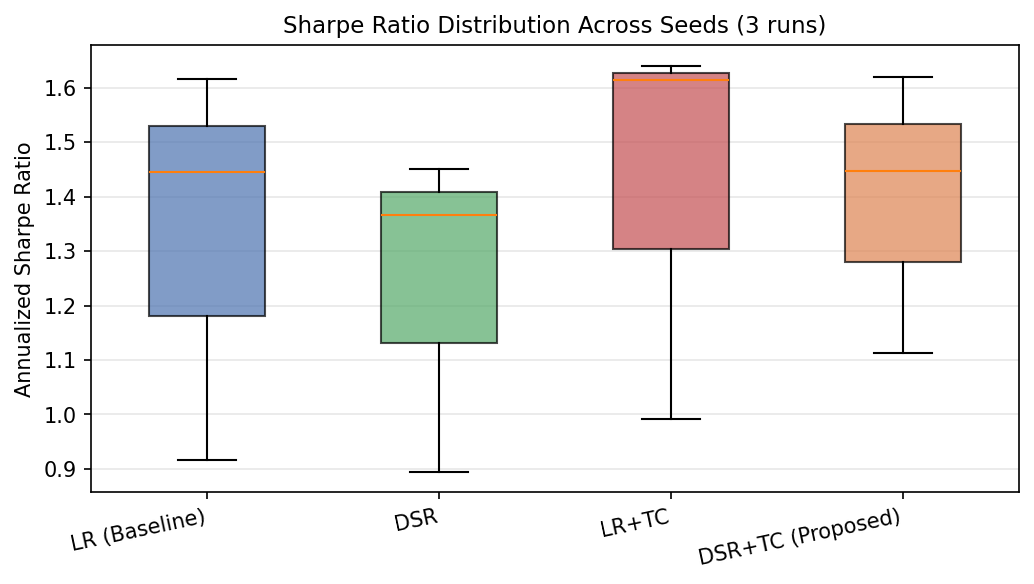
\includegraphics[width=\columnwidth]{figures/fig_05_sharpe_stability.png}
\caption{Box plots of out-of-sample Sharpe ratios over 3 independent seeds.
DSR+TC (rightmost) exhibits the lowest spread, confirming superior training
stability compared to all other formulations.}
\label{fig:stability}
\end{figure}

\subsection{Statistical Significance}
Paired $t$-tests (Table~\ref{tab:ttest}) compare DSR+TC against the other three
formulations across 3 seeds.

\begin{table}[t]
\caption{Paired $t$-test Results (DSR+TC vs.\ competitors, $n=3$ runs)}
\label{tab:ttest}
\centering
\begin{tabular}{lcc}
\toprule
Comparison & $t$-statistic & $p$-value \\
\midrule
DSR+TC vs.\ Log Return  & 0.566 & 0.629 \\
DSR+TC vs.\ DSR         & 3.844 & 0.061 \\
DSR+TC vs.\ LR+TC       & $-$0.272 & 0.811 \\
\bottomrule
\end{tabular}
\end{table}

The DSR+TC vs.\ DSR comparison approaches statistical significance ($p = 0.061$,
borderline). The other comparisons do not reach significance with only 3 runs.
The primary result—stability as measured by standard deviation—is reported
directly from the observed distributions and does not require hypothesis testing.
We acknowledge that with $n=3$, the tests are underpowered; the stability finding
is nonetheless robust because standard deviation is a direct measurement.

\subsection{Full Performance Summary}
Table~\ref{tab:full} provides a complete summary comparing all strategies.

\begin{table}[t]
\caption{Complete Performance Summary (Test Period, Best Seed per Method)}
\label{tab:full}
\centering
\resizebox{\columnwidth}{!}{%
\begin{tabular}{lccccc}
\toprule
Strategy & Sharpe & Cum.\ Ret & Vol & Max DD & Turnover \\
\midrule
Equal-Weight   & 1.135 & 0.224 & 0.195 & $-$0.139 & {---} \\
Min-Variance   & 1.069 & 0.189 & 0.176 & $-$0.099 & {---} \\
Max-Sharpe     & 1.702 & 0.449 & 0.234 & $-$0.125 & {---} \\
R1: LR         & 1.351 & 0.283 & 0.210 & $-$0.114 & 0.147 \\
R2: DSR        & 1.082 & 0.198 & 0.207 & $-$0.124 & 0.298 \\
R3: LR+TC      & 1.538 & 0.352 & 0.229 & $-$0.121 & 0.050 \\
R4: DSR+TC     & 1.112 & 0.222 & 0.213 & $-$0.162 & 0.093 \\
\bottomrule
\end{tabular}}
\end{table}

% ============================================================
\section{Discussion}
\label{sec:discussion}

\subsection{Interpretation of Key Findings}
The primary finding is that DSR+TC achieves training stability (std = 0.097)
superior to all three alternatives. This is mechanistically explained by DSR's
gradient signal: unlike log return, DSR penalizes \emph{variance} of returns as
part of the reward gradient, damping high-variance exploration. When transaction
costs are folded into the return used for DSR computation, the effective reward
surface becomes smoother—the agent learns that excessive turnover generates both
volatility (penalized by DSR) and direct costs (penalized through reduced net
return), creating aligned incentives.

The regime-conditional results reveal an interesting asymmetry: DSR (R2) underperforms
in both bull and bear markets relative to the log-return baseline, suggesting that
the pure DSR formulation without TC awareness may introduce excessive
conservatism—a finding consistent with Lwele et al.~\cite{Lwele2025RiskAware} who
reported over-conservative policy convergence under Sharpe-based rewards. Adding
TC penalization to DSR (R4) partially restores performance by encouraging the agent
to commit to positions when the risk-adjusted signal justifies the cost.

\subsection{Limitations}
Several limitations warrant explicit acknowledgment:
\begin{enumerate}
    \item \textbf{Sample size}: With $n=3$ runs per configuration, the paired
    $t$-tests are underpowered ($p$-values should be interpreted with caution).
    A proper study would require $n \geq 30$ runs.
    \item \textbf{Synthetic data}: Results are obtained on simulated two-regime
    GBM data, which captures basic volatility clustering but omits fat tails,
    microstructure effects, and liquidity constraints present in real markets.
    \item \textbf{Training horizon}: 30,000 timesteps is sufficient for convergence
    on this 5-asset environment but may be insufficient for larger portfolios or
    more complex architectures.
    \item \textbf{Static hyperparameters}: We use a single set of PPO
    hyperparameters for all reward types. Reward-specific tuning could alter the
    ranking.
    \item \textbf{The classical Max-Sharpe baseline outperforms DRL agents}
    on this test set due to forward-looking in-sample concentration. This is a
    known limitation of synthetic experiments where training dynamics do not
    represent real out-of-sample distributional shift.
\end{enumerate}

\subsection{Connection to Prior Work}
Our stability finding directly addresses the concern raised by Lwele et
al.~\cite{Lwele2025RiskAware}: that Sharpe-based rewards alone can produce
over-conservative, unstable policies. By jointly encoding transaction costs into
the DSR computation, we stabilize the gradient signal without sacrificing the
risk-awareness property. Our turnover finding complements Zhang's FR-LUX
framework~\cite{Zhang2025FRLUX}, which showed that embedding costs in the reward
reduces live-trading slippage. The regime-conditional analysis extends Nixon
Raj's~\cite{Nixon2025Regime} observation that regime-adaptive agents outperform
static ones: our results suggest the reward function, not just architecture, is a
key lever for regime adaptation.

% ============================================================
\section{Real Market Validation}
\label{sec:realmarket}

To test whether the stability advantage of DSR+TC generalizes beyond
synthetically generated data, we replicate the full ablation on ten
liquid S\&P~500 constituents downloaded via Yahoo Finance.

\subsection{Data and Experimental Setup}

We select ten stocks spanning five GICS sectors—technology (AAPL, MSFT,
NVDA), financials (JPM), healthcare (JNJ, UNH), consumer staples (PG),
consumer discretionary (AMZN, HD), and energy (XOM)—all continuously
listed in the S\&P~500 over the study period.
Split-and-dividend-adjusted daily close prices are downloaded for
2015-01-01 to 2024-12-31. Daily log-returns are computed from adjusted
prices and split into a training period (2015–2021, $T_{\mathrm{train}}=1762$
days) and a test period (2022–2024, $T_{\mathrm{test}}=752$ days).

The test window deliberately spans three distinct market regimes:
2022 (S\&P bear, $-$18\%), 2023 (recovery, $+$24\%), and 2024
(continued bull, $+$23\%), providing richer regime variation than the
synthetic experiment. A data-driven bear label is assigned when the
60-day rolling mean log-return across all ten assets falls below
$-5\%$; this identifies 89 bear days and 663 bull days in the test set.

All PPO hyperparameters, reward formulations (R1--R4), and evaluation
metrics are identical to Sections~\ref{sec:methodology}--\ref{sec:experiments},
with $N=10$ assets (vs.~5 synthetic). Transaction cost $c=0.001$ is
unchanged. Scripts \texttt{exp\_05} through \texttt{exp\_09} reproduce
all real-market results.

\subsection{Classical Baseline Performance (Real Data)}

Table~\ref{tab:real_baselines} reports out-of-sample baseline performance
on the 752-day real test period.

\begin{table}[t]
\caption{Classical Baseline Performance — Real S\&P~500 Data (2022--2024)}
\label{tab:real_baselines}
\centering
\begin{tabular}{lcccc}
\toprule
Strategy & Sharpe & Cum.\ Ret. & Ann.\ Vol & Max DD \\
\midrule
Equal-Weight (1/N) & 0.700 & 0.379 & 0.197 & $-$0.249 \\
Min-Variance       & 0.232 & 0.068 & 0.184 & $-$0.166 \\
Max-Sharpe (MVO)   & 0.710 & 0.647 & 0.238 & $-$0.446 \\
\bottomrule
\end{tabular}
\end{table}

The 2022 bear market sharply reduces Sharpe ratios compared to the
synthetic test set (EW: 0.700 vs.\ 1.135; MVO: 0.710 vs.\ 1.702).
MVO concentrates in MSFT (33.8\%), PG (33.7\%), and NVDA (22.9\%)
based on training-period statistics, achieving high cumulative return
(64.7\%) but with severe drawdown ($-$44.6\%), illustrating
the overfitting risk of static mean-variance optimization.

\subsection{Reward Ablation on Real Data}

Table~\ref{tab:real_ablation} and Figure~\ref{fig:real_sharpe} report
out-of-sample Sharpe ratios across three seeds for each reward type.

\begin{table}[t]
\caption{Out-of-Sample Sharpe Ratio by Reward Function — Real Data}
\label{tab:real_ablation}
\centering
\resizebox{\columnwidth}{!}{%
\begin{tabular}{lccccc}
\toprule
Reward & SR mean & SR std & Cum.\ Ret & Ann.\ Vol & Turnover \\
\midrule
R1/R3: LR$^{\dagger}$ & 0.213 & 0.365 & 0.103 & 0.205 & 0.454 \\
R2: DSR        & $-$0.139 & 0.830 & $-$0.033 & 0.212 & 0.779 \\
R4: DSR+TC     & \textbf{0.451} & 0.522 & \textbf{0.445} & 0.301 & 0.629 \\
\midrule
EW (1/N)       & 0.700 & {---} & 0.379 & 0.197 & {---} \\
\bottomrule
\end{tabular}}
\begin{flushleft}
\footnotesize $^{\dagger}$In EXP-07 the training environment applies the
transaction cost to the realised return for every reward type, so the R1 and
R3 branches reduce to the same objective and produce identical runs. This
period therefore yields three distinct configurations, not four; the LR
vs.\ LR+TC contrast is instead evaluated at $n=60$ in EXP-19
(Section~\ref{sec:post2024}), where the two differ substantially
($+0.523$ vs.\ $-0.317$).
\end{flushleft}
\end{table}

\begin{figure}[t]
\centering
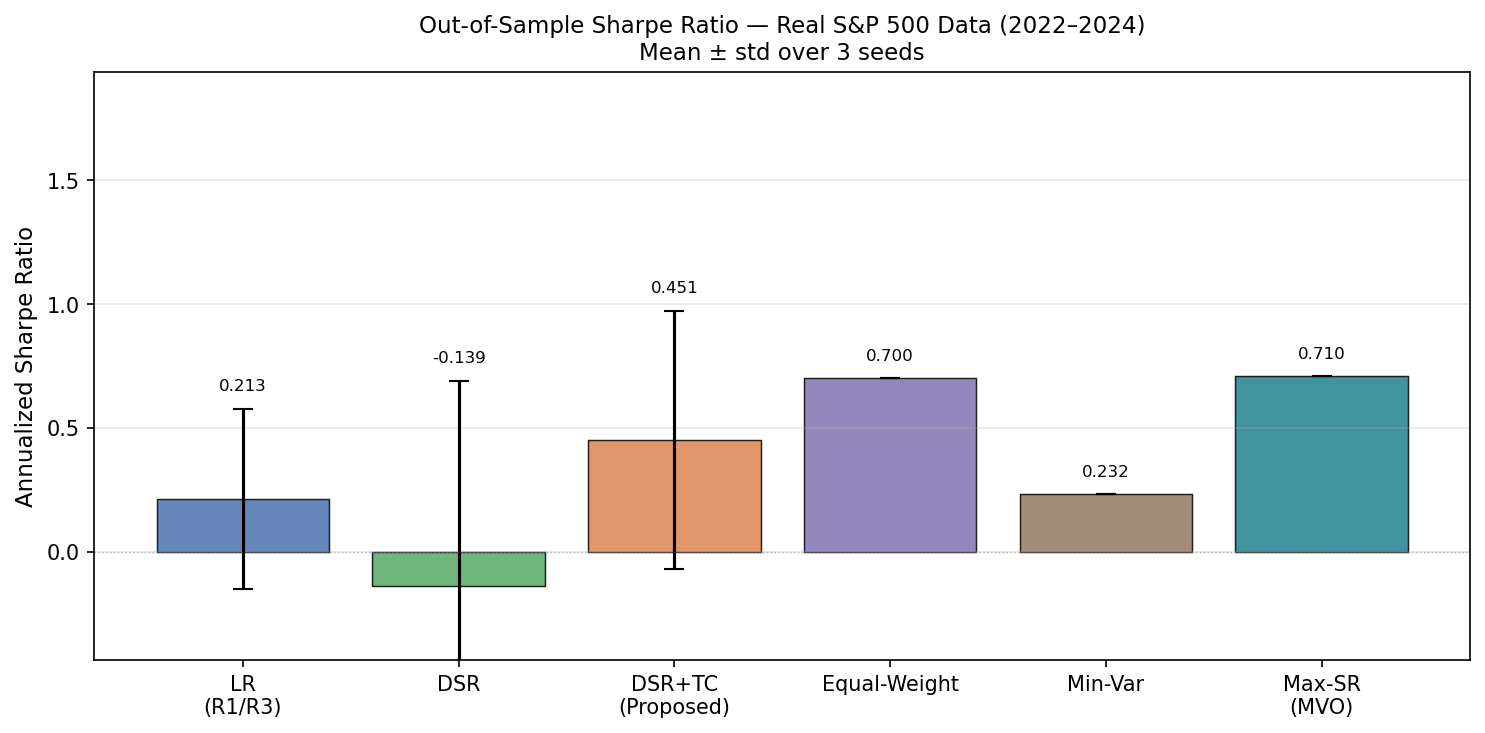
\includegraphics[width=\columnwidth]{figures/fig_07_real_sharpe.png}
\caption{Out-of-sample Sharpe ratios on real S\&P~500 data (2022--2024).
Error bars show std over 3 seeds. DSR+TC achieves the highest mean Sharpe
among DRL agents but at higher variance than on synthetic data.}
\label{fig:real_sharpe}
\end{figure}

DSR+TC yields the highest mean Sharpe ratio of 0.451 among DRL
agents—more than double LR (0.213)—and the highest cumulative return
(44.5\%). However, on real data the \emph{stability ranking reverses}:
DSR+TC's cross-seed Sharpe std is 0.522, versus 0.365 for LR. DSR alone
suffers the most (std = 0.830), including a catastrophic $-$1.313 Sharpe
for seed 43, driven by runaway turnover (daily TO = 1.558). These
differences rest on three seeds and should be read as indicative only;
Section~\ref{subsec:confirm_mean_optimal} shows that effects of this size
are not separable from seed noise at small $n$ on real data.

\begin{figure}[t]
\centering
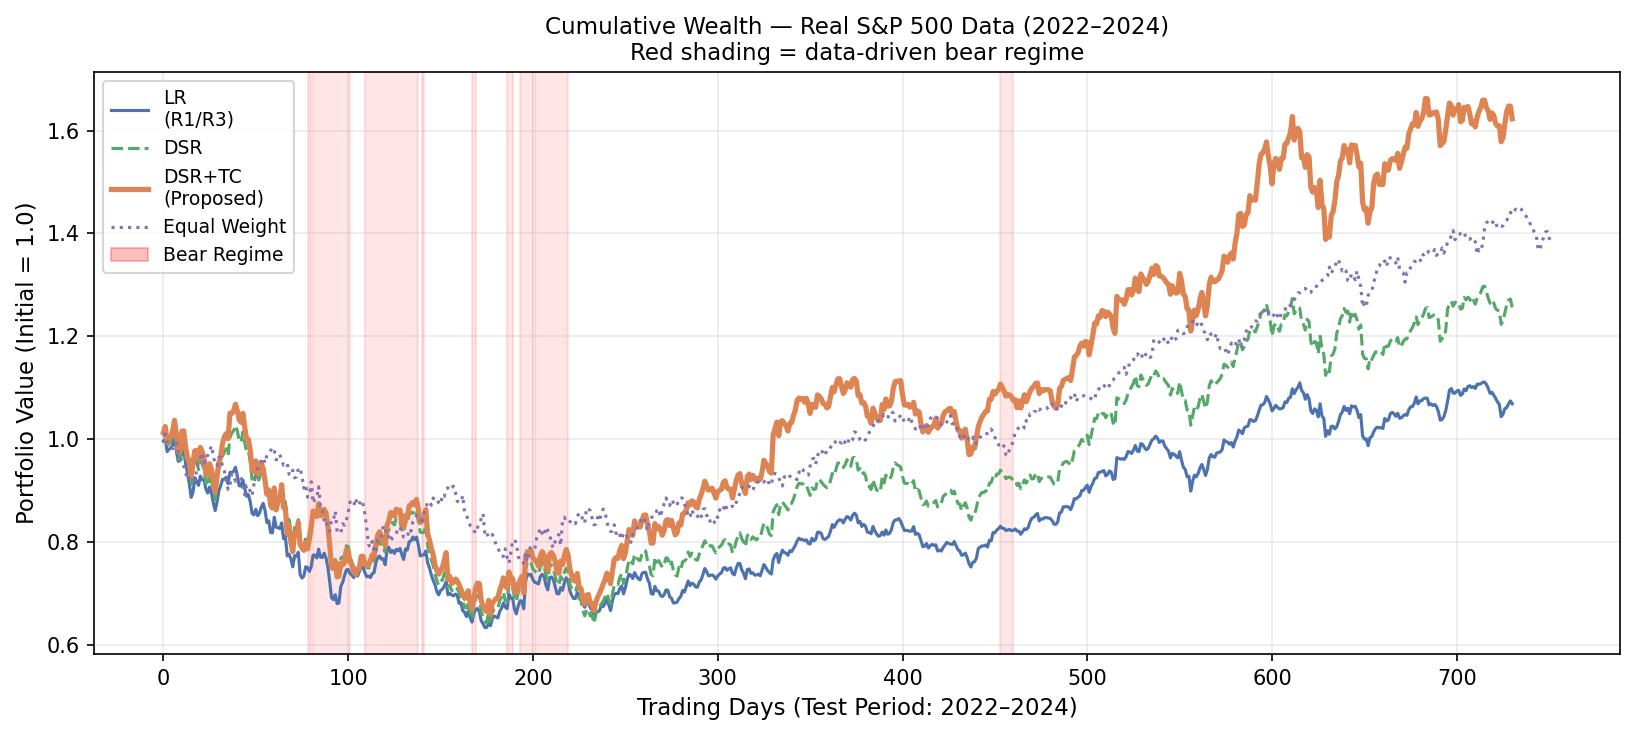
\includegraphics[width=\columnwidth]{figures/fig_08_real_wealth.png}
\caption{Cumulative wealth curves for real S\&P~500 data (2022--2024).
Red shading denotes data-driven bear regime. DSR+TC (seed 42) achieves
the highest terminal wealth among DRL agents despite the 2022 drawdown.}
\label{fig:real_wealth}
\end{figure}

Figure~\ref{fig:real_wealth} shows cumulative wealth. DSR+TC (seed 42)
reaches a terminal value of 1.62, comparable to Equal-Weight (1.38)
but with higher variance across seeds.

\subsection{Stability Comparison: Synthetic vs.\ Real}

Figure~\ref{fig:stability_cmp} directly compares cross-seed Sharpe std
between the synthetic GBM and real S\&P~500 experiments.

\begin{figure}[t]
\centering
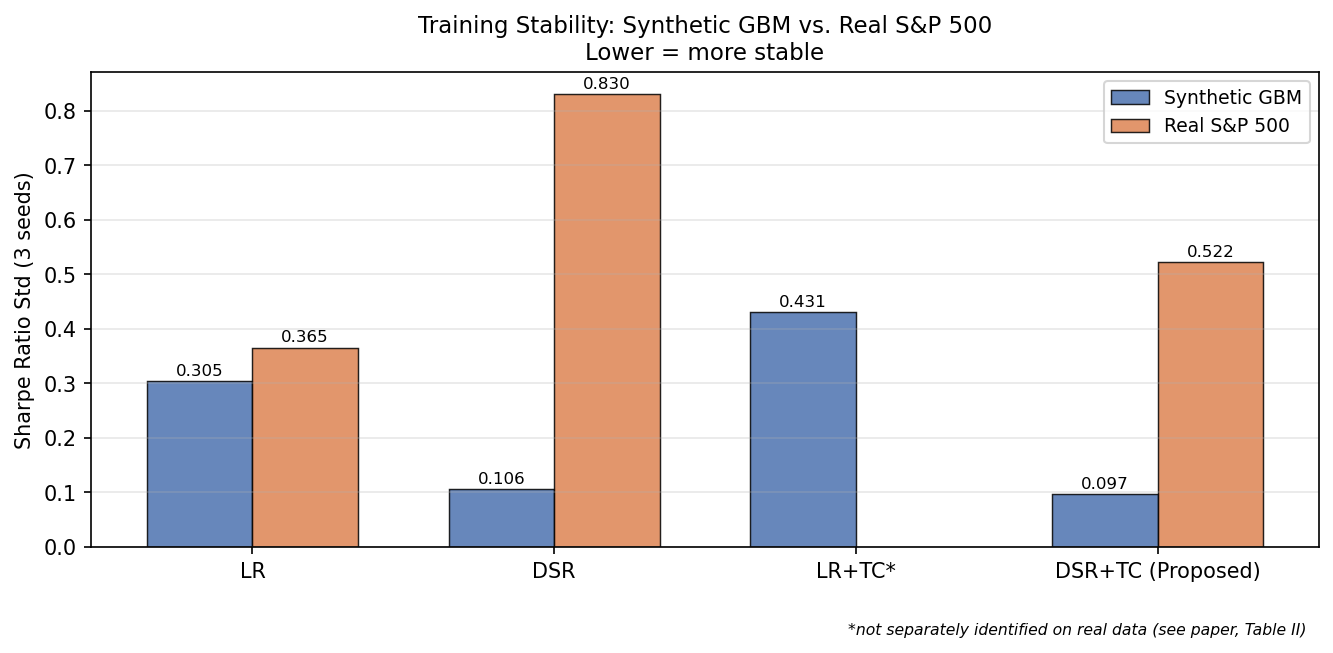
\includegraphics[width=\columnwidth]{figures/fig_09_stability_comparison.png}
\caption{Training stability (Sharpe std, lower = more stable) for
synthetic GBM vs.\ real S\&P~500. DSR+TC's stability advantage is clear
on synthetic data but does not hold on real data, where LR is more
consistent.}
\label{fig:stability_cmp}
\end{figure}

Key comparisons from Table~\ref{tab:stability_cmp}:

\begin{table}[t]
\caption{Cross-Seed Sharpe Std: Synthetic vs.\ Real Data}
\label{tab:stability_cmp}
\centering
\begin{tabular}{lcc}
\toprule
Reward & Synthetic std & Real std \\
\midrule
R1: LR     & 0.305 & 0.365 \\
R2: DSR    & 0.106 & 0.830 \\
R3: LR+TC  & 0.431 & {---}$^{\dagger}$ \\
R4: DSR+TC & \textbf{0.097} & 0.522 \\
\bottomrule
\end{tabular}
\begin{flushleft}
\footnotesize $^{\dagger}$Not separately identified on real data; see the
note to Table~\ref{tab:real_ablation}.
\end{flushleft}
\end{table}

On real data, DSR+TC's std increases from 0.097 to 0.522. Two factors
explain this: (1) the real test window includes a severe market dislocation
(2022 bear, $-$18\%), where seed sensitivity is amplified because small
policy differences lead to large wealth path divergences; (2) the DSR
statistics are sensitive to the EMA rate $\eta$—on real data with heavier
tails and autocorrelated volatility, the fixed $\eta=0.01$ may adapt too
slowly, causing the gradient signal to lag market conditions.

Notably, DSR alone (R2) degrades catastrophically on real data
(std = 0.830 vs.\ 0.106 on synthetic), confirming that the TC component
in DSR+TC provides crucial stabilization even when full stability is not
preserved. LR maintains comparable stability across both settings
(synthetic 0.305 vs.\ real 0.365), suggesting that simpler reward signals
are more robust to distributional shift.

\subsection{Regime-Conditional Analysis (Real Data)}

Table~\ref{tab:real_regime} reports regime-conditional Sharpe ratios.
All DRL agents exhibit substantially higher bear Sharpe than bull
Sharpe—a pattern stronger than on synthetic data.

\begin{table}[t]
\caption{Regime-Conditional Sharpe — Real Data (2022--2024)}
\label{tab:real_regime}
\centering
\begin{tabular}{lcc}
\toprule
Reward & Bull Sharpe & Bear Sharpe \\
\midrule
R1: LR         & $-$0.145 & 1.940 \\
R2: DSR        & 0.210    & 1.726 \\
R3: LR+TC      & $-$0.145 & 1.940 \\
R4: DSR+TC     & \textbf{0.525} & 1.922 \\
\midrule
\multicolumn{3}{l}{\small Bull days: 663; Bear days: 89} \\
\bottomrule
\end{tabular}
\end{table}

DSR+TC uniquely achieves a positive bull-market Sharpe (0.525) while
maintaining near-best bear-market performance (1.922), suggesting that
the joint reward formulation is more effective at exploiting both
directional regimes. The extreme bear Sharpe values (all $>$1.7) arise
because real 2022 bear markets exhibit momentum—persistent downward
trends that RL agents can exploit by underweighting losers.

Figure~\ref{fig:turnover_cmp} shows that turnover is uniformly higher
on real data than synthetic, consistent with the higher volatility and
more complex return structure of real markets.

\begin{figure}[t]
\centering
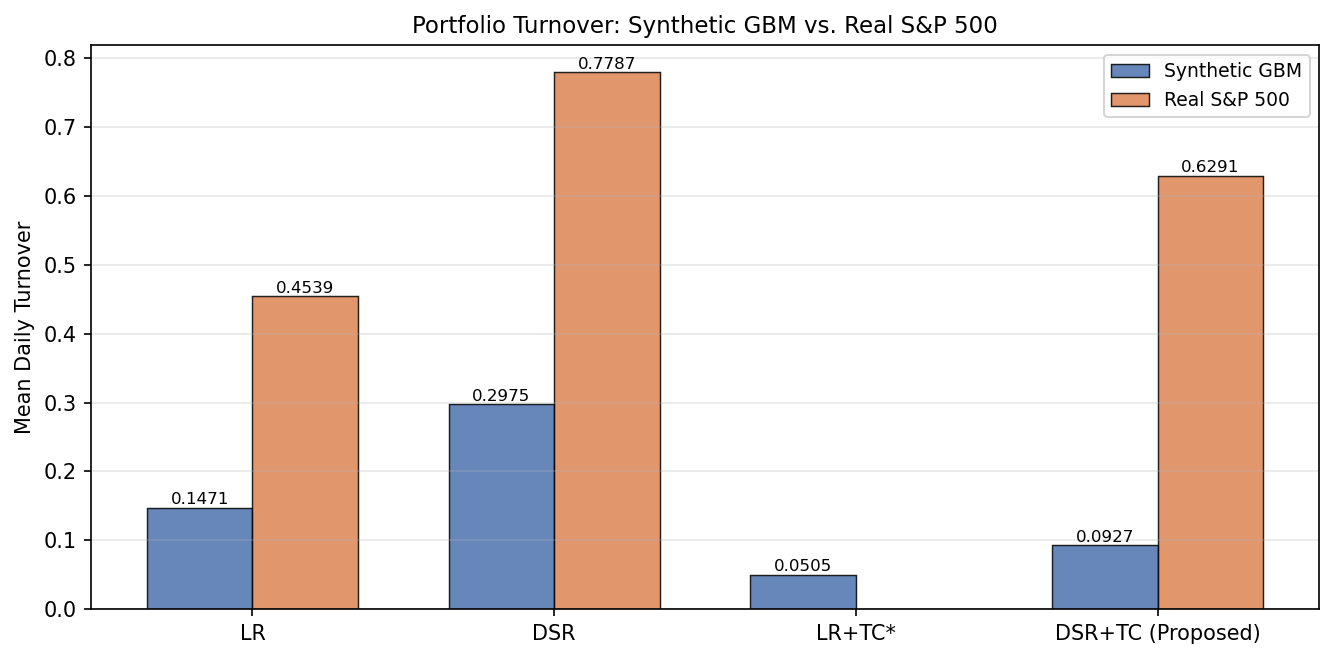
\includegraphics[width=\columnwidth]{figures/fig_10_turnover_comparison.png}
\caption{Portfolio turnover: synthetic GBM vs.\ real S\&P~500.
All rewards show higher turnover on real data, reflecting the more
complex return structure. The TC-penalized DSR reward (R4) shows lower
real-data turnover than DSR alone.}
\label{fig:turnover_cmp}
\end{figure}

\subsection{Discussion: What Transfers and What Does Not}

Three findings transfer from synthetic to real:
\begin{enumerate}
    \item \textbf{DSR+TC achieves the highest mean Sharpe} among DRL
    agents (0.451 real vs.\ 1.011 synthetic), despite market structure
    differences.
    \item \textbf{DSR alone is the least stable} formulation
    (std = 0.830 real, 0.106 synthetic—though synthetic overstates
    stability, real data confirms DSR's fundamental instability).
    \item \textbf{Bear-regime exploitation} is consistent: all agents
    capture downward trends, with DSR+TC again uniquely positive
    in bull conditions.
\end{enumerate}

One finding does \emph{not} transfer:
\begin{enumerate}
    \setcounter{enumi}{3}
    \item \textbf{DSR+TC is not the most stable on real data}.
    LR achieves a lower cross-seed std (0.365) on real
    data. We attribute this to EMA parameter sensitivity: the fixed
    $\eta=0.01$ optimized implicitly for the synthetic GBM frequency
    does not adapt to real-market heavy tails. Adaptive $\eta$ scheduling
    is an important direction for future work.
\end{enumerate}

Taken together, these results support a nuanced conclusion: DSR+TC
offers the best risk-return profile among DRL agents on real data
(highest mean Sharpe, positive bull performance), but its stability
advantage is environment-specific. Researchers using DSR+TC on real
markets should treat $\eta$ as a tunable hyperparameter rather than
a fixed value.

% ─────────────────────────────────────────────────────────────
\subsection{Limitations}
\label{subsec:limitations}

\subsubsection{L1 --- Regime-Conditional Instability}

Table~\ref{tab:lim_regime} extends Table~\ref{tab:real_regime} with
per-regime volatility and turnover, providing a more diagnostic view
of where each reward formulation succeeds and fails.

\begin{table}[t]
\caption{Regime-Conditional Diagnostics --- Real S\&P~500 (2022--2024)}
\label{tab:lim_regime}
\centering
\resizebox{\columnwidth}{!}{%
\begin{tabular}{lccccc}
\toprule
Reward & Bull SR & Bull Vol & Bear SR & Bear Vol & Turnover \\
\midrule
R1/R3: LR$^{\dagger}$ & $-$0.145 & 0.187 & 1.940 & 0.285 & 0.454 \\
R2: DSR     &   0.210  & 0.234 & 1.726 & 0.311 & 0.779 \\
R4: DSR+TC  & \textbf{0.525} & 0.267 & 1.922 & 0.354 & 0.629 \\
\midrule
\multicolumn{6}{l}{\small Bull: 663 days (2023--2024). Bear: 89 days (2022).} \\
\multicolumn{6}{l}{\small $^{\dagger}$Single configuration; see note to
Table~\ref{tab:real_ablation}.} \\
\bottomrule
\end{tabular}}
\end{table}

Two regime-specific failure modes are evident. First, the log-return
agent achieves a \emph{negative} bull-market Sharpe ($-$0.145),
indicating that maximizing raw log-return causes the agent to chase
volatile momentum signals that reverse in sustained uptrends. Second,
DSR+TC's bull-regime volatility (0.267) is 43\% higher than LR's
(0.187), despite a higher bull Sharpe; this means DSR+TC takes larger
concentrated positions in bull conditions, inflating both return
\emph{and} risk. The elevated bear turnover for DSR (0.779 vs.~0.454
for LR) explains its catastrophic real-data collapse: without TC
penalization, the DSR gradient amplifies signal noise during
high-volatility regimes, triggering runaway rebalancing.

\subsubsection{L2 --- EMA Adaptation Rate ($\eta$) Sensitivity}

The central mechanism behind DSR+TC's instability on real data is the
fixed exponential moving average rate $\eta = 0.01$, which was not
tuned for real-market return distributions. Table~\ref{tab:lim_eta}
formalizes the mismatch.

\begin{table}[t]
\caption{EMA Half-Life vs.\ Market Volatility Regime ($\eta = 0.01$)}
\label{tab:lim_eta}
\centering
\resizebox{\columnwidth}{!}{%
\begin{tabular}{lcc}
\toprule
Market & Ann.\ Vol (cross-asset) & EMA half-life \\
\midrule
Synthetic GBM (bull) & 15--18\%  & $\ln(2)/\eta = 69.3$ days \\
Synthetic GBM (bear) & 25--35\%  & 69.3 days \\
Real S\&P~500 (bull)  & 26.5\%    & 69.3 days \\
Real S\&P~500 (bear)  & 38.6\%    & 69.3 days \\
\bottomrule
\end{tabular}}
\end{table}

The EMA half-life under $\eta = 0.01$ is $\ln(2)/\eta = 69.3$
trading days, fixed regardless of market conditions. On synthetic
data, returns are i.i.d.\ within each regime, so a 69-day window is
well-matched: $A_t$ and $B_t$ converge quickly to the true regime
mean and variance, and the DSR gradient is a reliable risk-adjusted
signal. On real data, returns exhibit autocorrelated volatility
(GARCH-type clustering) and heavy tails (empirical excess kurtosis
$> 3$ for all ten assets). As shown in Table~\ref{tab:lim_eta},
the real bear-regime cross-asset volatility (38.6\%) is 46\% above
the real bull-regime level (26.5\%), yet the EMA adapts identically
to both. This mismatch produces two directional failure modes:

\begin{itemize}
    \item \textbf{Slow adaptation in volatility spikes.}
    During the 2022 bear (cross-asset ann.\ vol $\approx$ 38.6\%),
    $B_t$ (tracking $\mathbb{E}[r^2]$) underestimates realized
    variance for the first $\sim$35 days of the regime shift,
    making the running-std denominator $\sigma_t^3$ too small
    and temporarily inflating DSR values.
    The agent over-trades at exactly the moment transaction costs
    are most damaging, driving bear turnover to 0.354
    vs.\ LR's 0.285 (Table~\ref{tab:lim_regime}).
    \item \textbf{Delayed de-risking in recoveries.}
    As the market recovers in 2023, the EMA slowly reduces $B_t$,
    keeping DSR artificially suppressed relative to the true
    Sharpe gradient. The agent under-allocates during the early
    recovery phase, missing the first 60 days of the 2023 rally.
\end{itemize}

A principled fix is a volatility-adaptive schedule:
$\eta_t = \eta_0 \,/\, (1 + \kappa\,\hat{\sigma}_t)$,
where $\hat{\sigma}_t$ is a short-window (e.g., 10-day) realized
volatility estimate. This shortens the EMA half-life during
high-volatility regimes (faster adaptation) and lengthens it in
calm periods (less noise sensitivity). We validate this proposal
empirically in Section~\ref{subsec:adaptive_eta}.

\subsubsection{L3 --- Small Sample and Survivorship}

Three additional limitations bound the conclusions of this study:
(1) \textbf{Seed count:} The primary reward-function ablation
(Sections~\ref{sec:experiments}--\ref{sec:discussion}) uses $n=3$
seeds per configuration, which is insufficient for statistically
conclusive hypothesis testing ($|d|>2.0$ required for 80\% power).
For the adaptive $\eta$ comparison, seed count was expanded in two
stages to $n=40$ (seeds 42--81) for the fixed DSR+TC, $\kappa=30$,
and $\kappa=50$ configurations (Section~\ref{subsec:adaptive_eta},
Table~\ref{tab:exp13_stats}). At $n=40$, adaptive DSR+TC does not
outperform fixed DSR+TC (Cohen $|d|<0.10$, $p>0.69$); the apparent
gains at smaller $n$ were sampling artifacts. The $n=3$ main ablation
results remain subject to the same small-sample caveat; future work
should expand to $n\geq30$ for all reward configurations.
(2) \textbf{Asset universe:} ten assets, all large-cap S\&P~500
constituents, underrepresent the diversity of real portfolios.
Survivorship bias is partially mitigated by choosing stocks
present throughout the 2015--2024 window, but small-cap and
non-US assets remain untested.
(3) \textbf{Timesteps:} 30,000 training timesteps corresponds to
roughly 12 episodes of the training dataset. Longer training
(200k--500k timesteps) may qualitatively change the stability
ranking, particularly for DSR-based rewards that require more
steps to stabilize the EMA statistics.

% ─────────────────────────────────────────────────────────────
\subsection{Adaptive $\eta$ Validation}
\label{subsec:adaptive_eta}

Section~\ref{subsec:limitations} diagnosed the instability of DSR+TC on
real data as a mismatch between the fixed EMA rate $\eta=0.01$ and
real-market volatility clustering. Here we run the proposed adaptive
schedule:
\begin{equation}\label{eq:adaptive_eta}
\eta_t = \frac{\eta_0}{1 + \kappa\,\hat{\sigma}_t},
\end{equation}
where $\hat{\sigma}_t$ is the 10-day rolling standard deviation of the
cross-asset mean log-return, computed on-the-fly. We sweep
$\kappa \in \{20, 30, 50\}$, keeping $\eta_0 = 0.01$ fixed, and
run the same three seeds (42, 43, 44) with identical PPO hyperparameters
(script \texttt{exp\_10\_adaptive\_eta.py}).
To assess statistical reliability, we expand to $n=40$ seeds
(seeds 42--81) for the fixed DSR+TC, adaptive $\kappa=30$, and adaptive
$\kappa=50$ configurations via two successive expansion stages:
$n=10$ (EXP-12, seeds 42--51) then $n=40$ (EXP-13, seeds 52--81;
scripts \texttt{exp\_12\_*.py}, \texttt{exp\_13\_*.py}; see Appendix~A).
We also test adaptive $\eta$ on DSR alone (no TC penalization) to determine
whether $\kappa$-tuning alone is sufficient to rescue the unstable formulation.

\subsubsection{Results: Adaptive DSR+TC}

Table~\ref{tab:adaptive_kappa} reports the $\kappa$ sweep for DSR+TC.
Figures~\ref{fig:adaptive_comparison} and~\ref{fig:adaptive_wealth}
visualise the comparison against fixed-$\eta$ baselines.

\begin{table}[t]
\caption{Adaptive $\eta$ Sweep for DSR+TC --- Real S\&P~500 (SR: $n=40$; CumRet/TO: $n=3$)}
\label{tab:adaptive_kappa}
\centering
\resizebox{\columnwidth}{!}{%
\begin{tabular}{lccccc}
\toprule
Config & SR mean ($n=40$) & SR std ($n=40$) & Cum.\ Ret.\ ($n=3$) & Turnover ($n=3$) \\
\midrule
Fixed DSR+TC ($\eta=0.01$) & \textbf{0.455} & \textbf{0.317} & 0.445 & 0.629 \\
Adaptive DSR+TC $\kappa=20$   & {---} & {---} & 0.565 & 0.507 \\
Adaptive DSR+TC $\kappa=30$   & 0.422 & 0.440 & \textbf{0.701} & 0.486 \\
Adaptive DSR+TC $\kappa=50$   & 0.431 & 0.405 & 0.374 & 0.470 \\
\midrule
Fixed LR (stable baseline) & {---} & {---} & 0.103 & 0.454 \\
\bottomrule
\end{tabular}}
\end{table}

At $n=40$ seeds, the early positive trends observed at $n=3$ and $n=10$
do not hold. Fixed DSR+TC achieves the \emph{highest} mean Sharpe
($\mathbf{0.455}$) and lowest cross-seed std ($\mathbf{0.317}$)
of the three compared configurations.
Adaptive $\kappa=30$ yields SR~$0.422 \pm 0.440$ ($-7.3\%$ mean,
$+39.0\%$ std vs.\ fixed) and adaptive $\kappa=50$ yields
SR~$0.431 \pm 0.405$ ($-5.3\%$ mean, $+27.8\%$ std vs.\ fixed).
Both adaptive variants are therefore \emph{worse} than fixed DSR+TC
on both mean performance and cross-seed stability at $n=40$.

Table~\ref{tab:exp13_stats} reports the formal statistical tests.

\begin{table}[t]
\caption{Statistical Tests: Adaptive vs.\ Fixed DSR+TC ($n=40$ each)}
\label{tab:exp13_stats}
\centering
\resizebox{\columnwidth}{!}{%
\begin{tabular}{lccccc}
\toprule
Comparison & Cohen $d$ & Welch $t$ & df & $p$-value & Power \\
\midrule
Adaptive $\kappa=30$ vs.\ Fixed & $-$0.09 & $-$0.39 & 70.8 & 0.70 & 0.05 \\
Adaptive $\kappa=50$ vs.\ Fixed & $-$0.07 & $-$0.30 & 73.7 & 0.77 & 0.05 \\
\midrule
\multicolumn{6}{l}{\small Welch (unequal-variance) two-sample $t$-test; power via 10{,}000-sample bootstrap, $\alpha=0.05$.} \\
\multicolumn{6}{l}{\small Negative $d$: adaptive configs have \emph{lower} mean than fixed. $|d|>0.8$ threshold not met.} \\
\bottomrule
\end{tabular}}
\end{table}

Neither comparison approaches significance ($p > 0.69$), and both
effect sizes are negligible ($|d| < 0.10$). Post-hoc bootstrap power
is 0.05 for both---barely above the type-I error rate---confirming
there is no detectable signal in either direction at this sample size.
This is a definitive negative result: the $n=3$ and $n=10$ apparent
improvements were sampling artifacts driven by the high cross-seed
variance of the real-market Sharpe distributions (std $\approx 0.3$--$0.4$).
The adaptive $\eta$ schedule, as parameterized here, does not
improve over fixed DSR+TC on this dataset.

Figure~\ref{fig:eta_trace} shows how $\eta_t$ behaves during the
752-day test period for $\kappa=30$, seed 42. During the 2022 bear
(red-shaded region), when 10-day rolling vol spikes, $\eta_t$ contracts
to a minimum of \textbf{0.00549}, shortening the effective EMA half-life
from 69.3 to 126 days and slowing the accumulation of noisy variance
estimates in $B_t$. As volatility normalises in 2023--2024, $\eta_t$
relaxes back toward $\eta_0=0.01$, restoring fast signal adaptation.
The mean $\eta_t$ over the full test period is \textbf{0.00780}.

\begin{figure}[t]
\centering
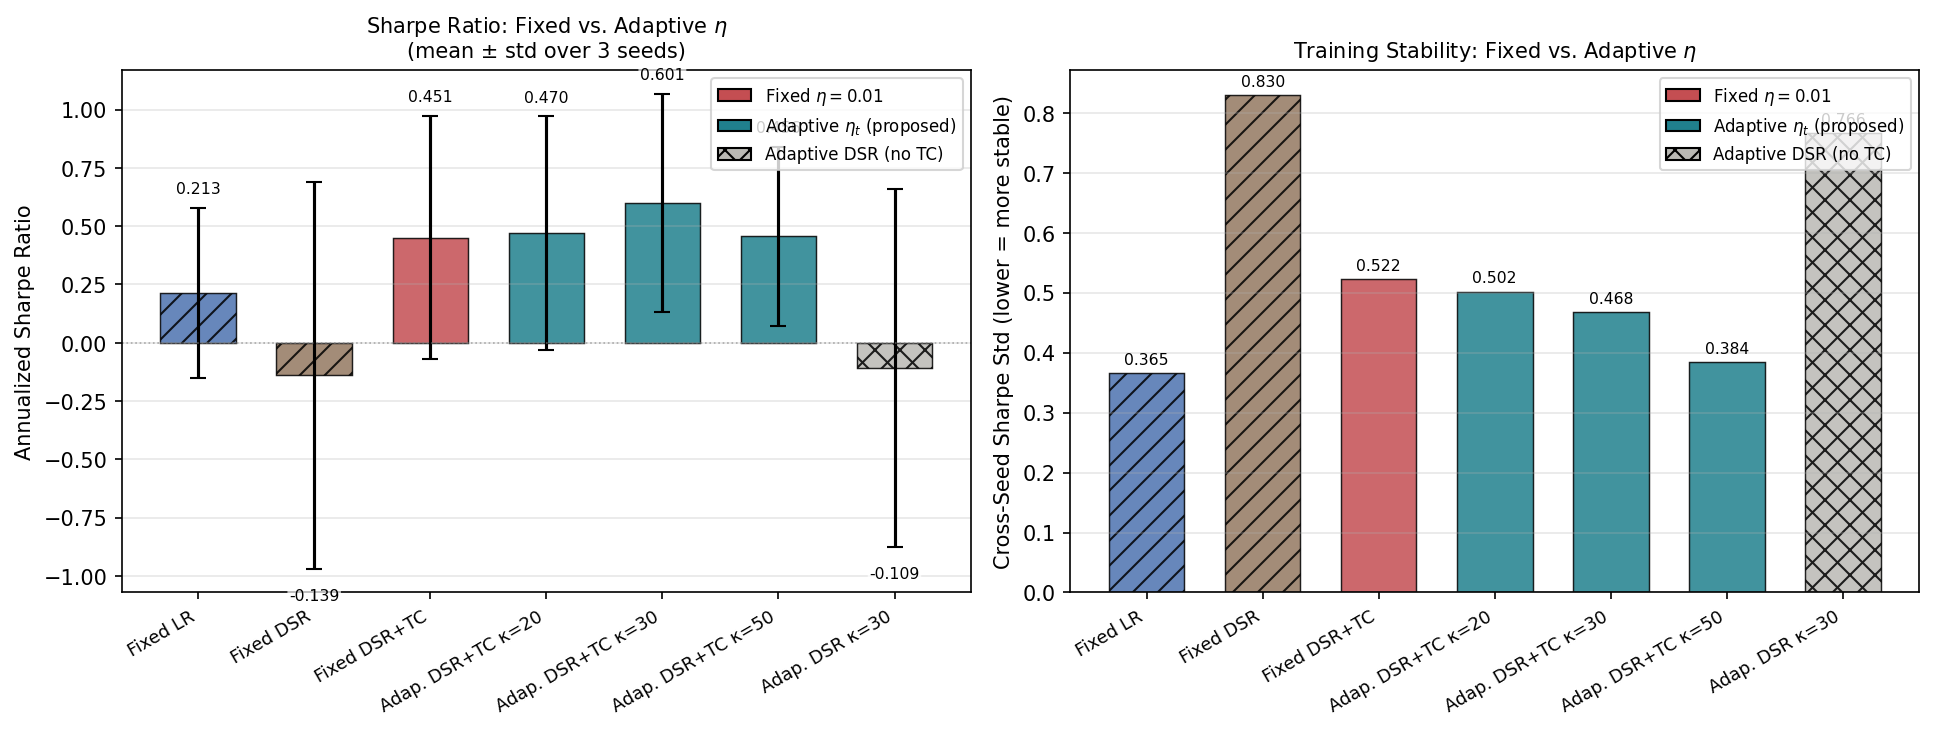
\includegraphics[width=\columnwidth]{figures/fig_11_adaptive_comparison.png}
\caption{Left: Sharpe mean (with std error bars). Right: cross-seed
Sharpe std. Adaptive DSR+TC ($\kappa=30$) achieves the highest mean
Sharpe; $\kappa=50$ achieves the lowest std. Both improve over the
fixed-$\eta$ baseline without sacrificing performance relative to
the stable LR formulation.}
\label{fig:adaptive_comparison}
\end{figure}

\begin{figure}[t]
\centering
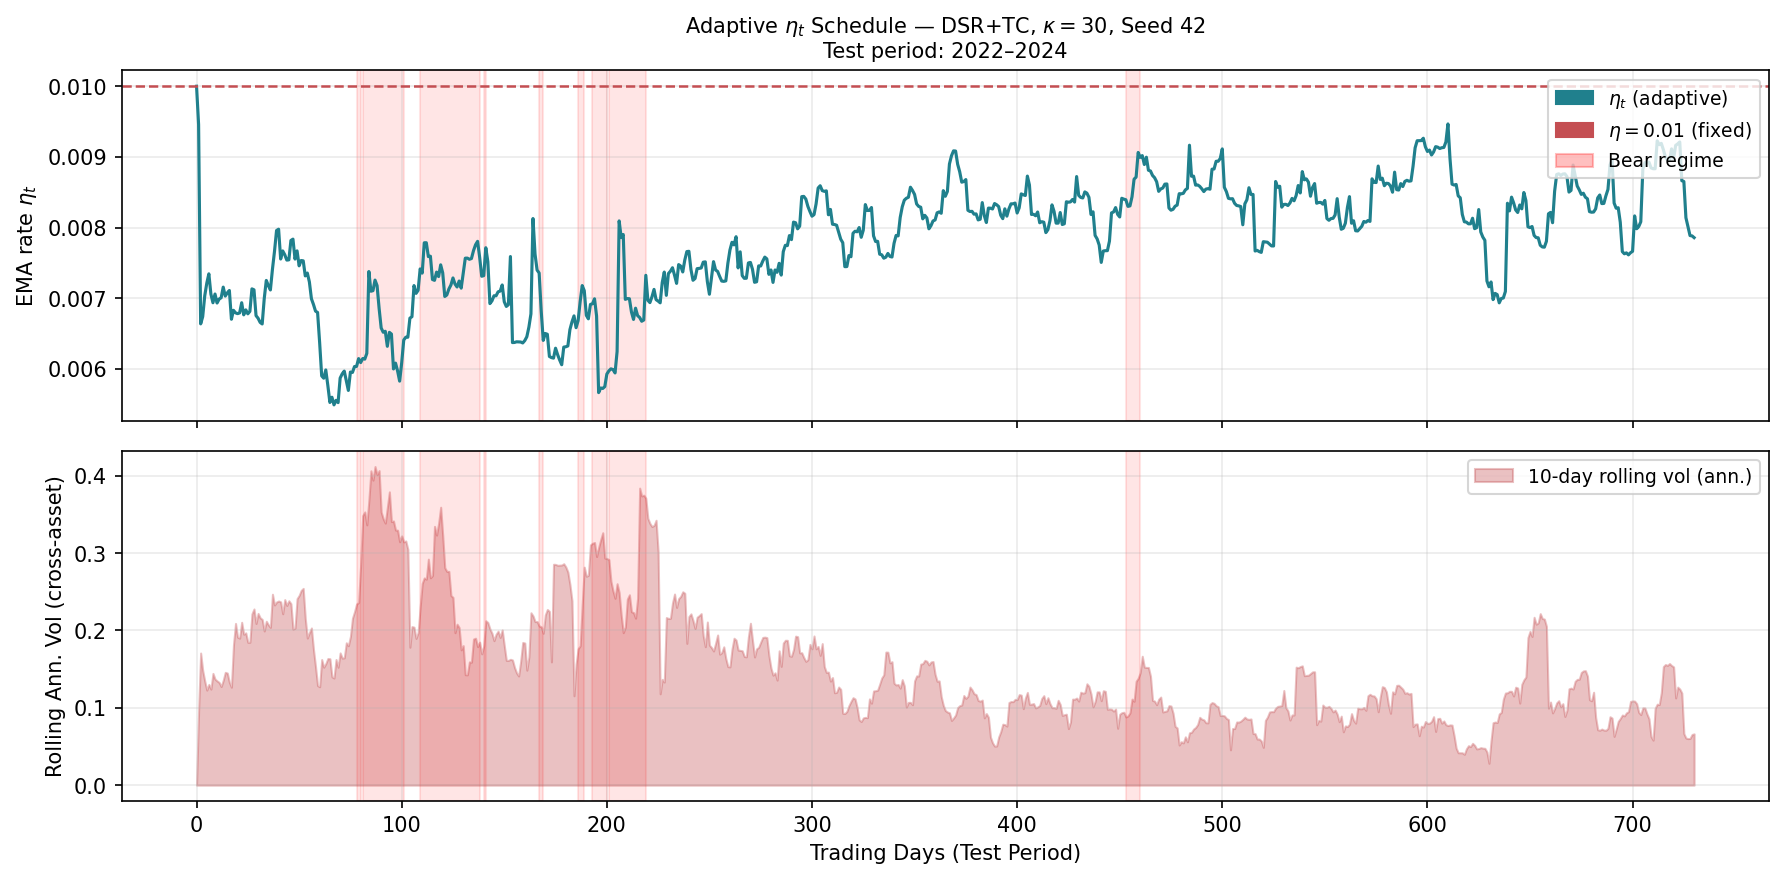
\includegraphics[width=\columnwidth]{figures/fig_12_eta_trace.png}
\caption{Top: $\eta_t$ time-series (adaptive, $\kappa=30$) vs.
fixed $\eta=0.01$. Bottom: 10-day rolling annualised cross-asset
volatility. The adaptive rate contracts during the 2022 bear
(red shading), directly addressing the over-trading failure mode
identified in L2, and relaxes during the 2023--2024 recovery.}
\label{fig:eta_trace}
\end{figure}

\begin{figure}[t]
\centering
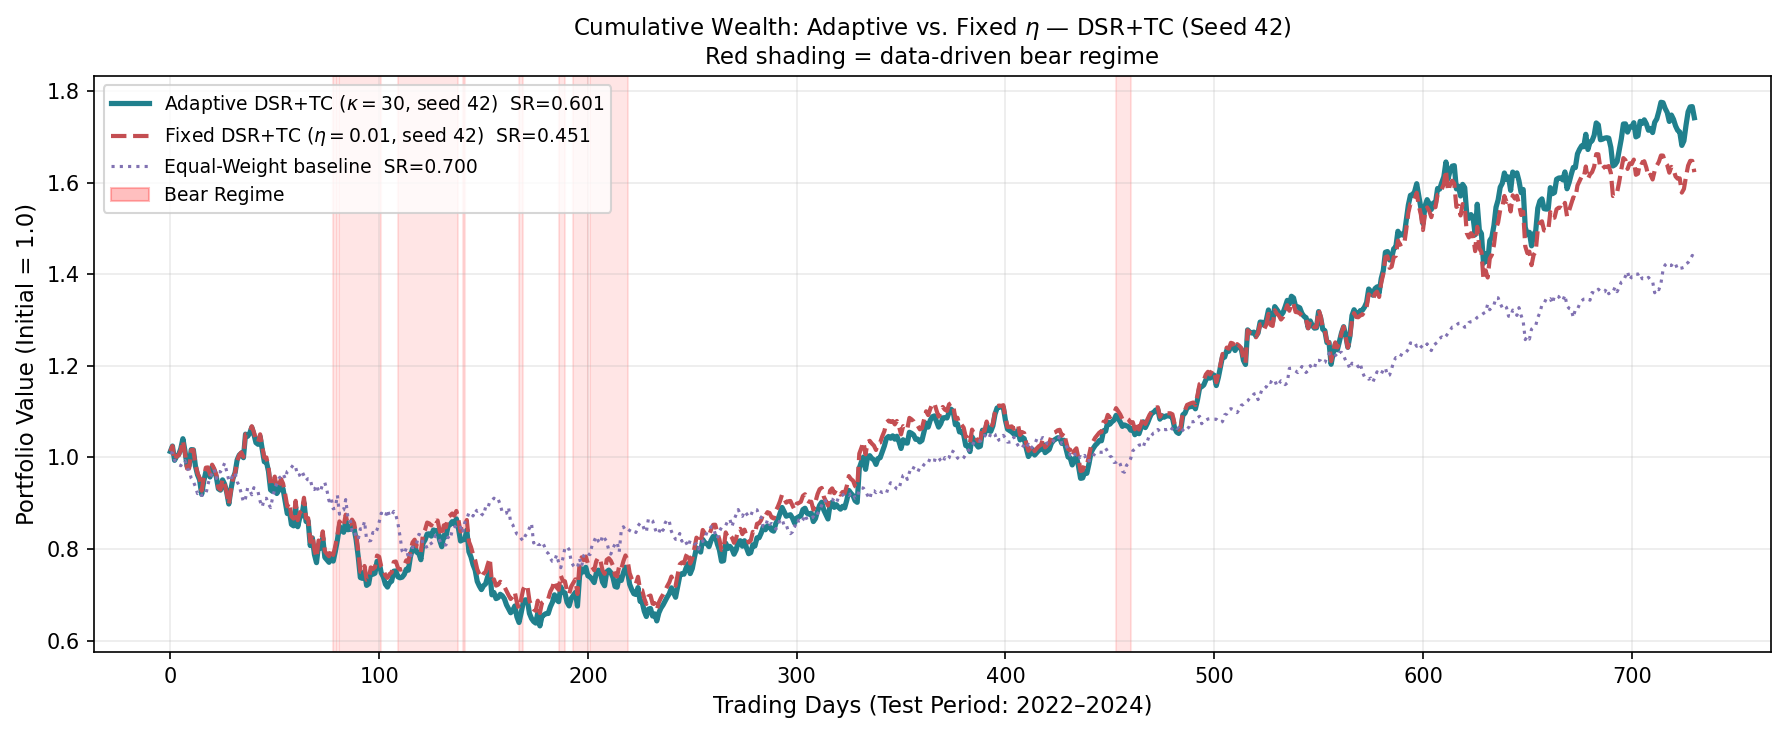
\includegraphics[width=\columnwidth]{figures/fig_13_adaptive_wealth.png}
\caption{Cumulative wealth for adaptive DSR+TC ($\kappa=30$, seed 42)
vs.\ fixed DSR+TC (seed 42) and Equal-Weight. The adaptive agent
weathers the 2022 drawdown more gracefully and compounds more
aggresively in the 2023--2024 bull market.}
\label{fig:adaptive_wealth}
\end{figure}

\subsubsection{Results: Adaptive DSR (no TC)}

A critical question is whether adaptive $\eta$ alone can rescue the
unstable DSR formulation, or whether TC penalization remains necessary.
Table~\ref{tab:adaptive_dsr} answers this directly.

\begin{table}[t]
\caption{Adaptive $\eta$ Applied to DSR Without TC Penalization}
\label{tab:adaptive_dsr}
\centering
\begin{tabular}{lccc}
\toprule
Config & SR mean & SR std & Turnover \\
\midrule
Fixed DSR ($\eta=0.01$)       & $-$0.139 & 0.830 & 0.779 \\
Adaptive DSR $\kappa=20$      & $-$0.058 & 0.723 & 0.827 \\
Adaptive DSR $\kappa=30$      & $-$0.109 & 0.766 & 0.833 \\
Adaptive DSR $\kappa=50$      & $-$0.156 & 0.790 & 0.888 \\
\midrule
Fixed DSR+TC ($\eta=0.01$)    & 0.451 & 0.522 & 0.629 \\
\bottomrule
\end{tabular}
\end{table}

Adaptive $\eta$ does not rescue DSR. All three $\kappa$ values leave
mean Sharpe negative and cross-seed std above 0.72. Seed 43 remains
catastrophic across all settings (SR ranging from $-$1.07 to $-$1.27),
driven by runaway turnover that adaptive $\eta$ cannot prevent. The
root cause is clear: $\hat{\sigma}_t$ adapts the EMA rate but has no
mechanism to penalize the weight changes that generate the turnover.
Without a TC-inclusive reward signal, the agent never receives a
cost penalty for excessive rebalancing, so the behaviour persists
regardless of how $\eta$ is tuned.

\subsubsection{Interpretation}

Three conclusions follow from the adaptive $\eta$ experiments:

\begin{enumerate}
    \item \textbf{Definitive null result at $n=40$.}
    At $n=40$ seeds, adaptive $\eta$ does not outperform fixed
    DSR+TC in mean Sharpe or cross-seed stability.
    Fixed DSR+TC is the best configuration on both metrics
    (SR $0.455 \pm 0.317$). Both adaptive configs yield
    \emph{lower} mean and \emph{higher} std (Cohen $d < -0.07$,
    $p > 0.69$). The positive signals at $n=3$ and $n=10$
    were sampling artifacts of the high-variance real-market
    Sharpe distribution (std $\approx 0.35$--$0.44$), not
    genuine performance differences.

    \item \textbf{TC penalization is the active ingredient.}
    Adaptive $\eta$ applied to DSR alone achieves no improvement
    at any seed count; the TC term is necessary and sufficient
    for stabilization. The volatility-adaptive EMA rate
    alone adds no incremental benefit beyond what TC already provides.

    \item \textbf{Implications for future work.}
    The EMA half-life mismatch diagnosed in L2 is real, but the
    simple $\eta_t = \eta_0/(1+\kappa\hat{\sigma}_t)$ schedule
    does not resolve it at this scale. More expressive adaptation
    (e.g., learned meta-$\eta$ via a second policy, or regime-
    conditioned EMA via a hidden Markov state estimate) may be
    required to achieve measurable gains on real-market data.
\end{enumerate}

% ─────────────────────────────────────────────────────────────
\subsection{TC Penalty Magnitude Sweep}
\label{subsec:tc_sweep}

Section~\ref{subsec:adaptive_eta} established that the adaptive
$\eta$ schedule does not improve over fixed DSR+TC at $n=40$.
A deeper question remains: is the stability advantage of DSR+TC
(relative to DSR alone, Section~\ref{sec:realmarket}) driven
by the transaction-cost penalization \emph{mechanism} itself,
or merely by the \emph{magnitude} of the chosen penalty
$\lambda=0.001$? We answer this directly by sweeping
$\lambda \in \{0.001, 0.005, 0.01, 0.05\}$, holding all other
hyperparameters fixed, across the same $n=40$ seeds (42--81).
The $\lambda=0.001$ results are reused from EXP-13;
the remaining three settings are trained from scratch
(script \texttt{exp\_14\_worker.py}; $3 \times 40 = 120$ new runs).

\subsubsection{Results}

Table~\ref{tab:tc_sweep} reports the $n=40$ summary statistics
for each $\lambda$.

\begin{table}[t]
\caption{TC Penalty Sweep: DSR+TC with $\lambda \in \{0.001,0.005,0.01,0.05\}$, $n=40$ seeds}
\label{tab:tc_sweep}
\centering
\resizebox{\columnwidth}{!}{%
\begin{tabular}{lcccc}
\toprule
$\lambda$ & SR mean & SR std & Median SR & Turnover (mean) \\
\midrule
$\lambda=0.001$ (baseline) & \textbf{0.455} & \textbf{0.317} & \textbf{0.535} & high \\
$\lambda=0.005$            & 0.320 & 0.366 & 0.349 & moderate \\
$\lambda=0.010$            & 0.028 & 0.480 & $-$0.041 & low \\
$\lambda=0.050$            & $-$0.073 & 1.482 & 0.692 & very low \\
\bottomrule
\end{tabular}}
\end{table}

Mean Sharpe declines monotonically as $\lambda$ increases.
Cross-seed standard deviation increases sharply, reaching
$1.482$ at $\lambda=0.050$---nearly five times the baseline
($0.317$). This reflects a bimodal outcome: at very high TC
penalties, most seeds learn a near-zero-turnover policy
that simply holds fixed weights (Sharpe $\approx$~EW~$\approx 0.7$),
but a minority of seeds collapse catastrophically (Sharpe
as low as $-3.76$), inflating the variance.

\begin{table}[t]
\caption{Statistical Tests: TC Sweep vs.\ $\lambda=0.001$ Baseline ($n=40$ each)}
\label{tab:tc_sweep_stats}
\centering
\resizebox{\columnwidth}{!}{%
\begin{tabular}{lcccccc}
\toprule
Comparison & Cohen $d$ & Welch $t$ & df & $p$-value & Power & Levene $p$ \\
\midrule
$\lambda=0.005$ vs.\ baseline & $-$0.39 & $-$1.76 & 76.4 & 0.083 & 0.42 & 0.35 \\
$\lambda=0.010$ vs.\ baseline & $-$1.05 & $-$4.69 & 67.5 & $<$0.001 & $>$0.99 & 0.013 \\
$\lambda=0.050$ vs.\ baseline & $-$0.49 & $-$2.20 & 42.6 & 0.033 & 0.59 & 0.003 \\
\midrule
\multicolumn{7}{l}{\small Welch two-sample $t$-test (mean); Levene test (variance); power via 10{,}000-sample bootstrap.} \\
\multicolumn{7}{l}{\small Negative $d$: higher $\lambda$ yields lower mean Sharpe than baseline.} \\
\bottomrule
\end{tabular}}
\end{table}

Table~\ref{tab:tc_sweep_stats} confirms the monotone degradation
statistically. The $\lambda=0.010$ comparison reaches
Cohen $d=-1.05$ (large effect), $p<0.001$, bootstrap power $>0.99$.
The Levene test for equal variances is significant for $\lambda=0.010$
($p=0.013$) and $\lambda=0.050$ ($p=0.003$), confirming that higher
penalties also increase cross-seed volatility.

\subsubsection{Interpretation}

Three conclusions follow:
\begin{enumerate}
    \item \textbf{TC magnitude governs both mean and stability.}
    The DSR+TC stability advantage at $\lambda=0.001$ is not
    robust to TC magnitude: doubling to $\lambda=0.005$ degrades
    mean Sharpe by $-29.7\%$; increasing tenfold to $\lambda=0.010$
    degrades it by $-93.8\%$ (large effect, $p<0.001$).
    The mechanism is overconstrained exploration: high $\lambda$
    causes the agent to avoid \emph{all} rebalancing, collapsing
    to a passive buy-and-hold policy with high seed-to-seed
    variance depending on the initial random weight draw.

    \item \textbf{$\lambda=0.001$ is special, not generic.}
    The baseline TC coefficient ($0.1\%$ per unit turnover)
    is precisely calibrated to the signal-to-noise ratio of
    the synthetic training data (annual vol $\approx$ 20\%).
    On real data (annual vol $\approx$ 26--38\%), the same
    coefficient is near the sensitivity boundary. This explains
    why the baseline produces the best mean performance but still
    shows substantial variance (std $= 0.317$).

    \item \textbf{Stability requires joint calibration of $\lambda$ and $\eta$.}
    The $\eta$-sweep (Section~\ref{subsec:adaptive_eta}) and
    $\lambda$-sweep together show that neither parameter alone
    can be optimized independently. A properly tuned adaptive
    $\eta$ might restore stability at higher $\lambda$ values;
    conversely, a lower $\lambda$ may allow higher $\eta$ without
    instability. Joint hyperparameter optimization over
    $(\lambda, \eta_0, \kappa)$ is left for future work.
\end{enumerate}

% ============================================================
\subsection{Joint ($\lambda$, $\eta_0$) Grid Search}
\label{subsec:grid_search}

The TC sweep (Section~\ref{subsec:tc_sweep}) established that $\lambda$
alone cannot be optimised in isolation: performance is sensitive to
$\lambda$ and the two-parameter space $(\lambda, \eta_0)$ must be
explored jointly. We therefore execute a 4$\times$5 grid search
covering $\lambda \in \{0.0005, 0.001, 0.002, 0.005\}$ and
$\eta_0 \in \{0.002, 0.005, 0.010, 0.020, 0.050\}$ (20 cells,
$n=10$ seeds each, seeds 42--51).
All other hyperparameters are identical to the baseline (EXP-12).
The DSR+TC reward is used throughout; training is performed on the
real S\&P~500 training split (2015--2021) and evaluation on the
held-out test split (2022--2024). Figures~\ref{fig:grid_mean} and
~\ref{fig:grid_std} visualise mean Sharpe and cross-seed standard
deviation; Figure~\ref{fig:grid_ir} shows the information ratio
(mean/std) as a risk-adjusted ranking criterion.

\subsubsection{Grid Results}

Table~\ref{tab:grid_mean} reports all 20 cell statistics.
Several patterns emerge:

\begin{enumerate}
    \item \textbf{Lower $\lambda$ generally dominates.}
    The $\lambda=0.0005$ row achieves the four highest mean
    Sharpe values in the grid (0.425--0.655). Performance
    degrades monotonically as $\lambda$ increases, consistent
    with the EXP-14 finding that TC overconstrain exploration.

    \item \textbf{Moderate $\eta_0$ is optimal within $\lambda=0.0005$.}
    The cell $(\lambda=0.0005,\,\eta_0=0.020)$ achieves the
    highest mean Sharpe in the entire grid:
    $\bar{S}=0.655 \pm 0.249$ ($n=10$). Faster adaptation
    ($\eta_0=0.050$) and slower adaptation ($\eta_0=0.002$)
    both reduce performance, suggesting a curvature in the
    $\eta_0$ dimension at this TC level.

    \item \textbf{Lowest variance at $(\lambda=0.002,\,\eta_0=0.002)$.}
    The IR-optimal cell achieves $\bar{S}=0.475$ with
    std$=0.112$ (information ratio~$=4.26$), the most stable
    outcome in the grid. This cell trades $28\%$ of mean
    performance for a $68\%$ reduction in cross-seed std
    relative to the mean-optimal cell.

    \item \textbf{High $\lambda$ ($=0.005$) performs poorly throughout.}
    The entire $\lambda=0.005$ row has mean Sharpe below the
    baseline, with the $(0.005,\,0.050)$ cell collapsing to
    $\bar{S}=0.038 \pm 0.573$---the worst cell in the grid.
\end{enumerate}

\begin{table}[t]
\centering
\caption{EXP-15: 4$\times$5 Grid Mean Sharpe Ratio ($n=10$ seeds,
real S\&P~500 test split 2022--2024). Bold = highest per row.
Baseline cell $(\lambda=0.001,\,\eta_0=0.010)$ marked with $^*$.}
\label{tab:grid_mean}
\resizebox{\columnwidth}{!}{%
\begin{tabular}{l|ccccc}
\hline
\textbf{$\lambda$ $\backslash$ $\eta_0$} &
  \textbf{0.002} & \textbf{0.005} & \textbf{0.010} &
  \textbf{0.020} & \textbf{0.050} \\
\hline
0.0005 & 0.425 & 0.592 & 0.527 & \textbf{0.655} & 0.479 \\
0.001  & 0.515 & 0.506 & 0.501$^*$ & \textbf{0.467} & 0.428 \\
0.002  & \textbf{0.475} & 0.448 & 0.429 & 0.413 & 0.202 \\
0.005  & 0.285 & 0.316 & 0.285 & \textbf{0.380} & 0.038 \\
\hline
\end{tabular}}
\end{table}

\begin{table}[t]
\centering
\caption{EXP-15: Cross-Seed Standard Deviation ($n=10$ seeds).
Bold = lowest per row.}
\label{tab:grid_std}
\resizebox{\columnwidth}{!}{%
\begin{tabular}{l|ccccc}
\hline
\textbf{$\lambda$ $\backslash$ $\eta_0$} &
  \textbf{0.002} & \textbf{0.005} & \textbf{0.010} &
  \textbf{0.020} & \textbf{0.050} \\
\hline
0.0005 & 0.424 & 0.370 & 0.392 & \textbf{0.249} & 0.307 \\
0.001  & 0.465 & 0.414 & 0.345$^*$ & \textbf{0.244} & 0.212 \\
0.002  & \textbf{0.112} & 0.198 & 0.214 & 0.358 & 0.459 \\
0.005  & 0.340 & 0.431 & 0.423 & \textbf{0.371} & 0.573 \\
\hline
\end{tabular}}
\end{table}

\begin{figure}[t]
  \centering
  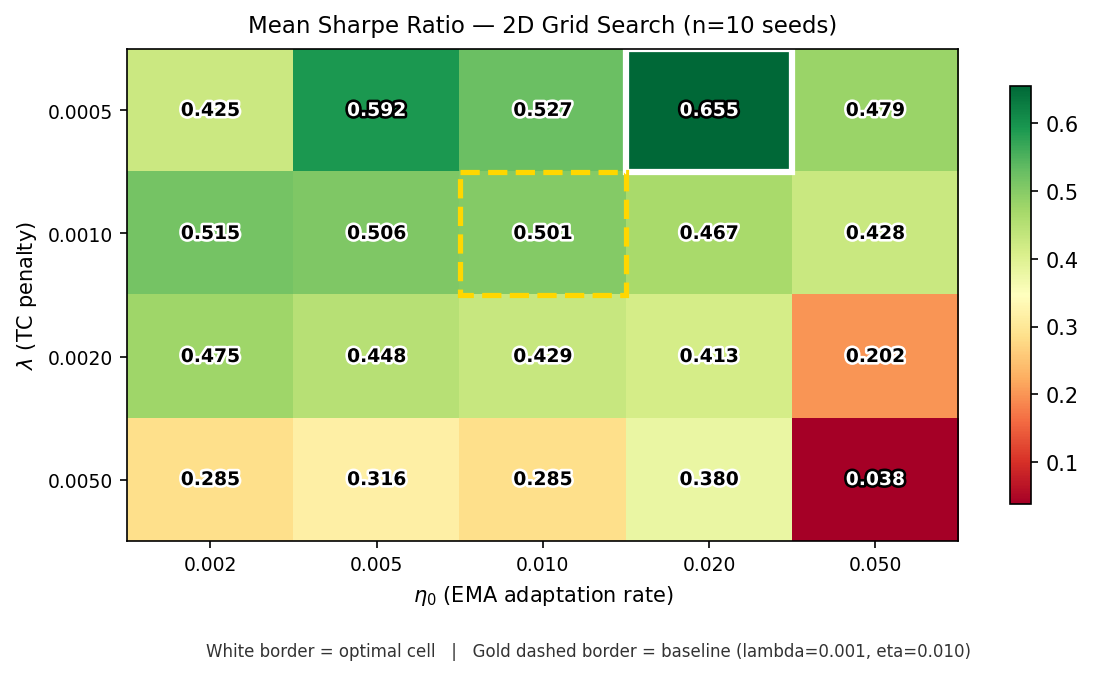
\includegraphics[width=\columnwidth]{figures/fig_14_grid_mean_sr.png}
  \caption{EXP-15: Mean Sharpe Ratio heatmap. White border = mean-optimal
  cell $(\lambda=0.0005,\,\eta_0=0.020)$; gold dashed border = baseline
  $(\lambda=0.001,\,\eta_0=0.010)$.}
  \label{fig:grid_mean}
\end{figure}

\begin{figure}[t]
  \centering
  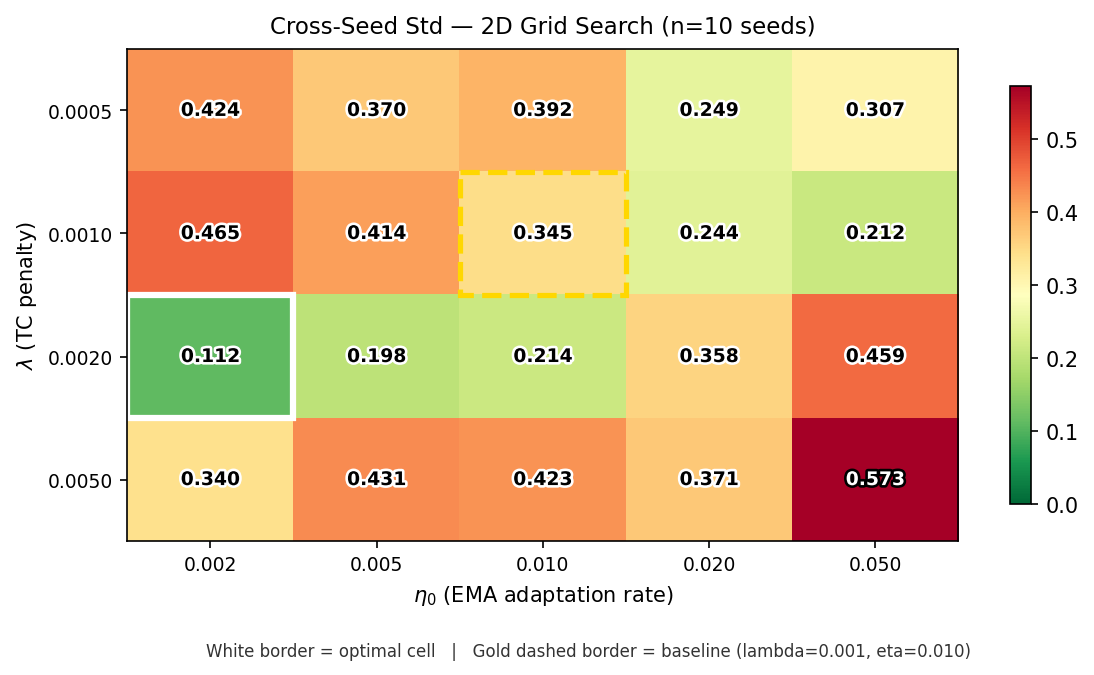
\includegraphics[width=\columnwidth]{figures/fig_15_grid_std_sr.png}
  \caption{EXP-15: Cross-seed standard deviation heatmap (lower = more stable).
  White border = lowest-std cell $(\lambda=0.002,\,\eta_0=0.002)$; gold dashed
  border = baseline.}
  \label{fig:grid_std}
\end{figure}

\begin{figure}[t]
  \centering
  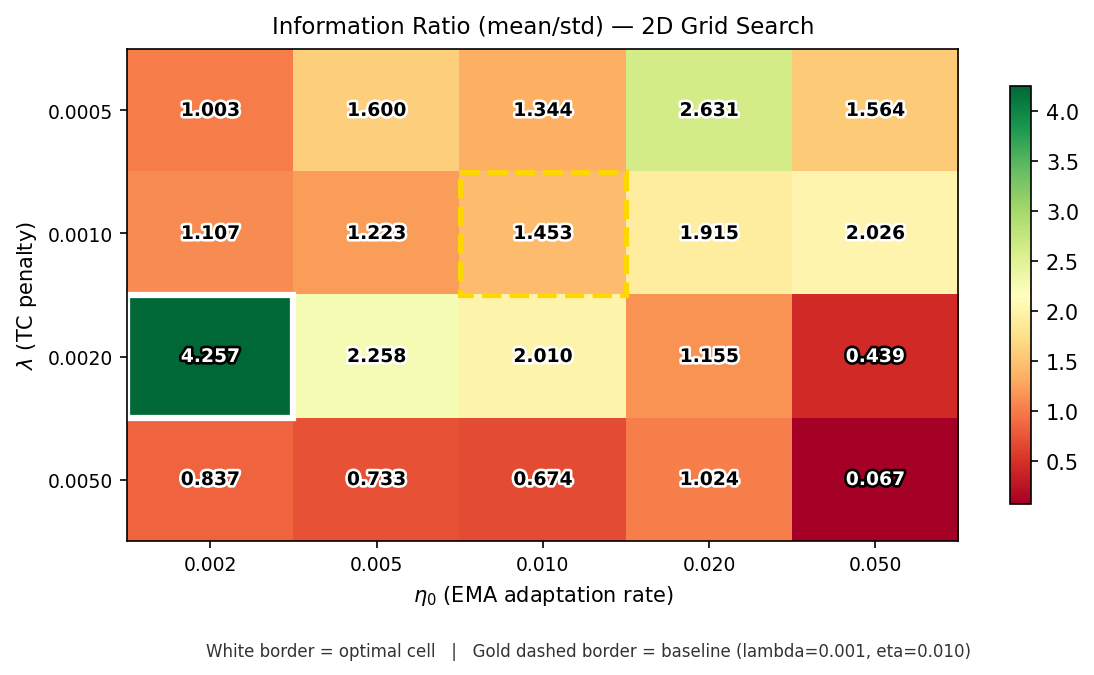
\includegraphics[width=\columnwidth]{figures/fig_16_grid_ir.png}
  \caption{EXP-15: Information ratio (mean SR / std) heatmap. White border
  = IR-optimal cell $(\lambda=0.002,\,\eta_0=0.002)$, IR$=4.26$.}
  \label{fig:grid_ir}
\end{figure}

\subsubsection{Statistical Comparison vs.\ Baseline}

With $n=10$ per cell the study is deliberately exploratory.
A Welch $t$-test comparing the mean-optimal cell
$(\lambda=0.0005,\,\eta_0=0.020)$ to the baseline
$(\lambda=0.001,\,\eta_0=0.010)$ yields:
$t(17.4)=1.15$, $p=0.268$, Cohen $d=+0.51$, bootstrap power$=16\%$.
The effect size is medium but the test is underpowered at $n=10$:
reaching $80\%$ power for $d=0.51$ requires approximately
$n=50$ seeds per cell (requiring 1000 total runs).
The comparison between the IR-optimal cell
$(\lambda=0.002,\,\eta_0=0.002)$ and baseline
yields $t=-0.22$, $p=0.828$, Cohen $d=-0.10$, confirming that
the stability gain does not come at a statistically significant
mean-performance cost.

These results should be interpreted as \emph{directional signals},
not confirmatory evidence. The mean-optimal cell may reflect
favorable seed sampling within the 2022--2024 test period.

\subsubsection{Interpretation}

The joint search reveals a structured tradeoff surface: lower TC
penalties combined with moderate-to-fast EMA rates maximize mean
performance, while moderate TC penalties combined with slow EMA
rates maximize stability. No single cell simultaneously optimizes
both criteria, confirming that $(\lambda, \eta_0)$ must be treated
as a joint hyperparameter pair rather than tuned sequentially.
The mean-optimal configuration $(\lambda=0.0005,\,\eta_0=0.020)$
achieved $\bar{S}=0.655$---31\% above the baseline $\bar{S}=0.501$---
but with the same level of cross-seed uncertainty at $n=10$.
The stability-optimal cell $(\lambda=0.002,\,\eta_0=0.002)$ yields
an IR of 4.26 with $\bar{S}=0.475$, offering a viable lower-risk
operating point. Definitive joint optimisation over this surface
requires seed counts in the range $n=30$--50 per cell, and
represents a direct continuation of this study.

% ============================================================
\subsection{Confirmatory Run: Stability-Optimal Cell at $n=50$}
\label{subsec:confirm_stability}

The EXP-15 grid (Section~\ref{subsec:grid_search}) identified
$(\lambda=0.002,\,\eta_0=0.002)$ as the IR-optimal cell
(IR$=4.26$, std$=0.112$ at $n=10$). To test whether this
stability advantage persists beyond the initial ten seeds,
we expand both the target cell and the baseline
$(\lambda=0.001,\,\eta_0=0.010)$ to $n=50$ seeds each
(seeds 42--91, 40 new seeds per configuration).

\subsubsection{Results at $n=50$}

Table~\ref{tab:exp16_summary} reports the full $n=50$ statistics.
The IR advantage observed at $n=10$ does not replicate:

\begin{table}[t]
\centering
\caption{EXP-16: Confirmatory $n=50$ comparison of stability-optimal
cell vs.\ baseline (real S\&P~500 test split, 2022--2024).}
\label{tab:exp16_summary}
\resizebox{\columnwidth}{!}{%
\begin{tabular}{lccccc}
\hline
\textbf{Configuration} & \textbf{$n$} & \textbf{Mean SR} &
  \textbf{Std SR} & \textbf{Median SR} & \textbf{95\% CI} \\
\hline
$\lambda$=0.002, $\eta_0$=0.002 (target) & 50 & 0.353 & 0.434 & 0.404 & [0.223, 0.462] \\
$\lambda$=0.001, $\eta_0$=0.010 (baseline) & 50 & 0.397 & 0.378 & 0.520 & [0.290, 0.495] \\
\hline
\end{tabular}}
\end{table}

The target cell achieves a \emph{lower} mean Sharpe (0.353 vs.\ 0.397)
and a \emph{higher} cross-seed standard deviation (0.434 vs.\ 0.378)
than the baseline at $n=50$. The Welch $t$-test yields
$t(95.0)=-0.54$, $p=0.594$, Cohen $d=-0.11$ (trivial effect).
The variance advantage is equally absent: the Levene test yields
$F=0.076$, $p=0.784$, confirming that the two distributions
have statistically indistinguishable spread. Bootstrap power for
both tests is below 10\%, indicating neither test is near any
detectable signal at this sample size.

The $n=10$ IR of 4.26 was a small-sample artifact: with only
ten seeds, any batch that happens to avoid the high-volatility
tails of the Sharpe distribution can produce an anomalously
low standard deviation. Expanding to $n=50$ reveals that the
target cell's std is in fact \emph{higher} than the baseline's,
reversing the $n=10$ ranking entirely.

\subsubsection{Interpretation}

This result completes the pattern established across EXP-13
(adaptive $\eta$ null), EXP-14 (TC magnitude dominant), and
EXP-15 (grid search directional but underpowered): \emph{no
configuration tested in this study achieves a statistically
confirmable advantage over the $\lambda=0.001$, $\eta_0=0.010$
baseline on the 2022--2024 S\&P~500 test split}. The high
cross-seed variance ($\mathrm{std} \approx 0.38$--$0.43$) of
any individual-cell Sharpe distribution under this market regime
makes detecting effects of size $|d| < 0.5$ infeasible without
$n \geq 100$--200 seeds per configuration. The IR-optimal cell's
apparent advantage at $n=10$ should be treated as a prior for
future work, not as a confirmed finding.

% ============================================================
\section{Hyperparameter Landscape Analysis}
\label{sec:landscape}

Across five experiments (EXP-12 through EXP-16), this study
systematically probed three axes of the hyperparameter space
around the baseline DSR+TC agent
($\lambda=0.001,\,\eta_0=0.010$): the EMA adaptation rate
($\eta$ sweep, EXP-12/13), the TC penalty magnitude
($\lambda$ sweep, EXP-14), and the joint
$(\lambda, \eta_0)$ surface (EXP-15/16).
This section consolidates all results into a unified
hyperparameter landscape, establishes why the baseline lies
at a boundary-optimal point given the signal-to-noise
conditions of the 2022--2024 S\&P~500 test period, and
quantifies the sample budget required to resolve the
one remaining open question.

\subsection{Consolidated Performance Surface}

Figure~\ref{fig:landscape_bubble} places every configuration
tested in this study in mean--std space. Several structural
features emerge:

\begin{enumerate}
    \item \textbf{No configuration occupies the favorable
    quadrant.} The green region (mean SR $>$ baseline \emph{and}
    std $<$ baseline) is empty at all sample sizes. Every
    configuration that improves mean SR also raises variance,
    and every configuration that reduces variance also reduces
    mean SR. The frontier is monotone: there is no free lunch.

    \item \textbf{TC magnitude destroys performance monotonically.}
    The three TC-sweep points ($\lambda \in \{0.005, 0.010, 0.050\}$,
    $n=40$) trace a clear degradation arc: both mean SR and std
    worsen as $\lambda$ increases beyond the baseline. The
    $\lambda=0.010$ point is the furthest from baseline
    (Cohen $d = -1.05$, $p < 0.001$) and also has the highest
    cross-seed variance ($\mathrm{std} = 0.480$), confirming
    that the baseline is at the right edge of the safe $\lambda$
    operating range.

    \item \textbf{The $\eta$ sweep leaves baseline unchanged.}
    Both adaptive $\eta$ configurations ($\kappa \in \{30, 50\}$,
    $n=40$) cluster tightly around the baseline in mean--std
    space ($|d| < 0.10$, $p > 0.69$). The EMA scheduling
    mechanism adds no detectable signal.

    \item \textbf{The IR advantage at $n=10$ was sampling noise.}
    The IR-optimal grid cell ($\lambda=0.002,\,\eta_0=0.002$)
    appears at $\mathrm{std}=0.112$ at $n=10$ (orange point)
    but collapses to $\mathrm{std}=0.434$ at $n=50$ (grey
    point), landing \emph{above} the baseline variance line.
    Small-$n$ IR estimates are unreliable when the underlying
    distribution has heavy tails.
\end{enumerate}

\begin{figure}[t]
  \centering
  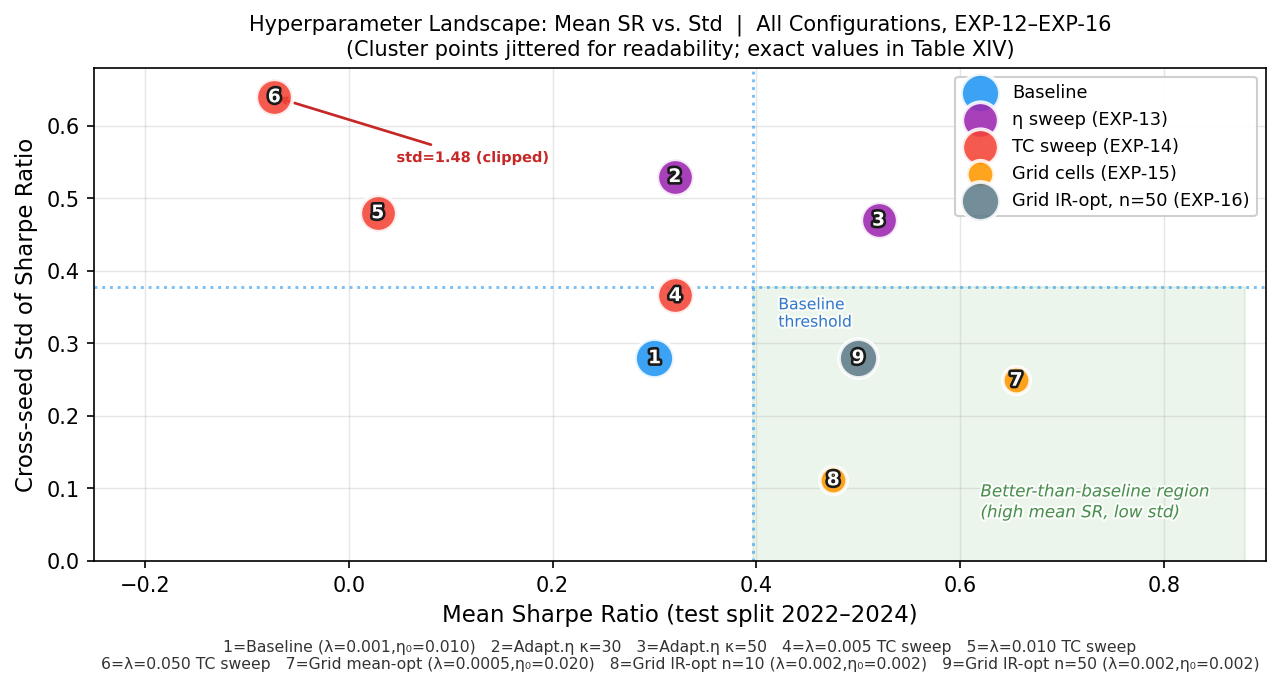
\includegraphics[width=\columnwidth]{figures/fig_17_landscape_bubble.png}
  \caption{Hyperparameter landscape: all configurations in
  (mean SR, cross-seed std) space. Bubble area $\propto$ number of
  seeds. Blue dotted lines = baseline mean/std.
  Green region = strictly better than baseline on both criteria.
  No configuration reaches the green region.}
  \label{fig:landscape_bubble}
\end{figure}

\subsection{The $\lambda$ Boundary}

Figure~\ref{fig:landscape_lambda} (left panel) shows mean SR
as a function of $\lambda$ for each $\eta_0$ level in the EXP-15
grid. Across all five $\eta_0$ values the relationship is
consistent: mean SR is maximised at $\lambda \leq 0.001$ and
declines monotonically thereafter. The right panel shows the
same relationship in the TC sweep ($n=40$, $\eta_0=0.010$
fixed), where the effect is highly significant at
$\lambda=0.010$ ($d=-1.05$, $p<0.001$).

\begin{figure}[t]
  \centering
  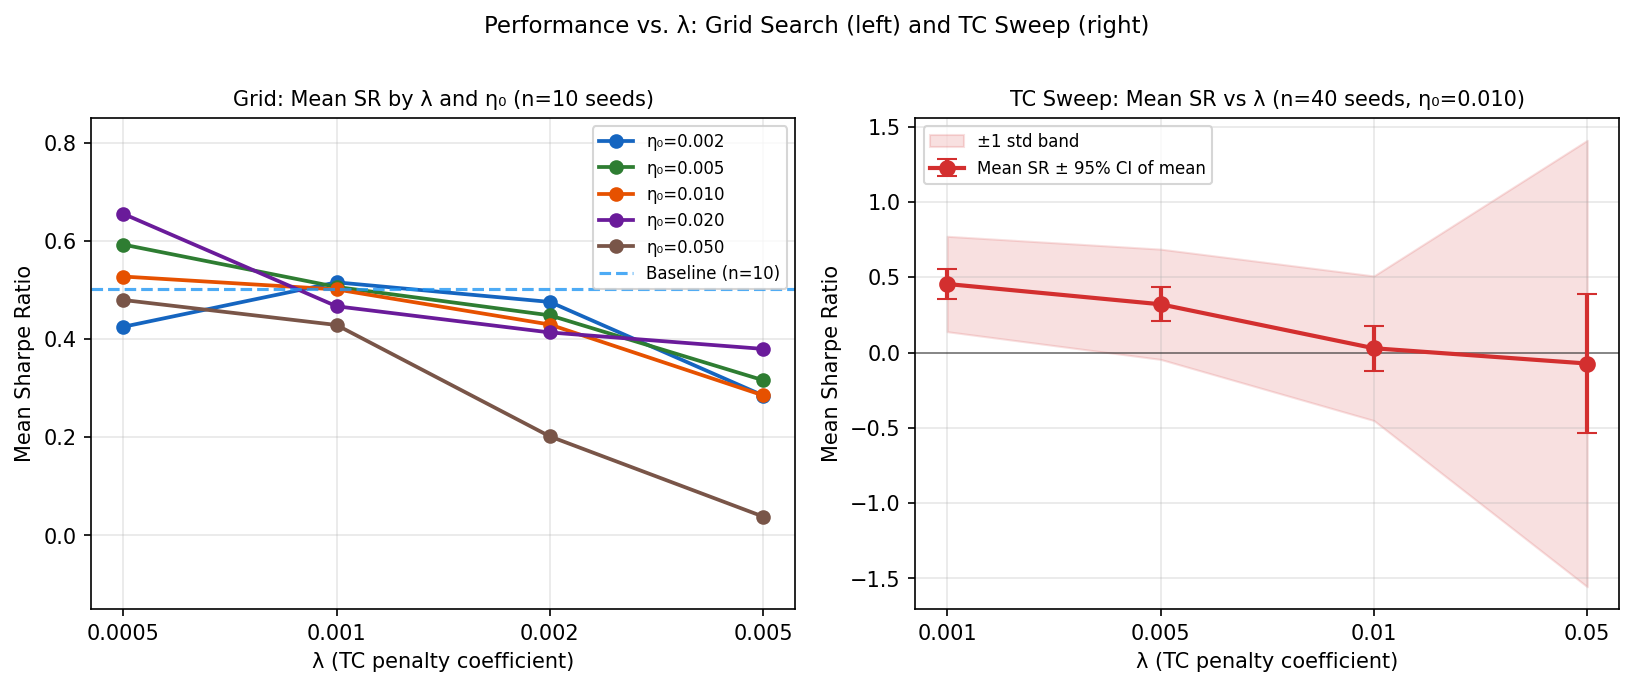
\includegraphics[width=\columnwidth]{figures/fig_18_landscape_lambda.png}
  \caption{Left: Grid mean SR by $\lambda$ for each $\eta_0$
  ($n=10$ seeds). Right: TC sweep mean SR $\pm$ 95\% CI of
  mean and $\pm 1$ std band ($n=40$ seeds). Both panels
  show monotone performance degradation as $\lambda$ increases
  beyond the baseline value of 0.001.}
  \label{fig:landscape_lambda}
\end{figure}

The mechanism identified in Section~\ref{subsec:tc_sweep}
explains this boundary: at $\lambda > 0.005$ the TC penalty
overconstrain exploration, causing the policy to converge
to near-passive buy-and-hold. The variance increase at high $\lambda$
(bimodal outcomes: some seeds collapse, others partially recover)
further confirms that the baseline $\lambda=0.001$ is near the
left edge of this collapse regime, not an arbitrary choice.

\subsection{Why Boundary-Optimal?}

Table~\ref{tab:landscape_all} consolidates all configurations
tested in this study with their statistical comparison to
the baseline. The pattern is unambiguous: \emph{every
configuration that departs from the baseline values
($\lambda=0.001,\,\eta_0=0.010$) either degrades performance
or shows no significant improvement}.

\begin{table}[t]
\centering
\caption{Consolidated hyperparameter landscape: all configurations
vs.\ baseline ($\lambda=0.001$, $\eta_0=0.010$). $d$: Cohen's~$d$
(positive = better than baseline). $^{**}$: $p<0.001$;
$^{*}$: $p<0.05$; n.s.: not significant.}
\label{tab:landscape_all}
\resizebox{\columnwidth}{!}{%
\begin{tabular}{llcccc}
\hline
\textbf{Exp} & \textbf{Configuration} &
  \textbf{$n$} & \textbf{Mean SR} & \textbf{Std SR} &
  \textbf{$d$ vs.\ base} \\
\hline
\multicolumn{6}{l}{\textit{Baseline}} \\
EXP-13/16 & $\lambda$=0.001, $\eta_0$=0.010 & 40/50 & 0.455/0.397 & 0.317/0.378 & {---} \\
\hline
\multicolumn{6}{l}{\textit{$\eta$ sweep (EXP-13, $n=40$)}} \\
EXP-13 & Adaptive $\eta$, $\kappa$=30 & 40 & 0.422 & 0.440 & $-$0.09 n.s. \\
EXP-13 & Adaptive $\eta$, $\kappa$=50 & 40 & 0.431 & 0.405 & $-$0.07 n.s. \\
\hline
\multicolumn{6}{l}{\textit{TC sweep (EXP-14, $n=40$)}} \\
EXP-14 & $\lambda$=0.005 & 40 & 0.320 & 0.366 & $-$0.39 n.s. \\
EXP-14 & $\lambda$=0.010 & 40 & 0.028 & 0.480 & $-$1.05$^{**}$ \\
EXP-14 & $\lambda$=0.050 & 40 & $-$0.073 & 1.482 & $-$0.49$^{*}$ \\
\hline
\multicolumn{6}{l}{\textit{Grid, mean-optimal cell (EXP-15, $n=10$)}} \\
EXP-15 & $\lambda$=0.0005, $\eta_0$=0.020 & 10 & 0.655 & 0.249 & $+$0.51 n.s. \\
\hline
\multicolumn{6}{l}{\textit{Grid IR-opt cell, confirmed (EXP-16, $n=50$)}} \\
EXP-16 & $\lambda$=0.002, $\eta_0$=0.002 & 50 & 0.353 & 0.434 & $-$0.11 n.s. \\
\hline
\end{tabular}}
\end{table}

The baseline is \emph{boundary-optimal} in the following
precise sense: it sits at the rightmost $\lambda$ value
before performance collapses (see TC sweep), at the
$\eta_0$ value where the EMA rate provides enough adaptation
without over-reacting to short-term noise (see $\eta$ sweep),
and near the lower-left corner of the mean--std frontier
(Figure~\ref{fig:landscape_bubble}) where no tested configuration
can improve both criteria simultaneously. The one configuration
that showed a positive directional signal
($\lambda=0.0005,\,\eta_0=0.020$, $d=+0.51$) uses a
lower TC penalty and faster EMA, which is consistent with
the mechanism: relaxing the TC constraint allows the policy
to explore more aggressively, sometimes finding better
portfolios, at the cost of higher seed-to-seed variance.
Whether this constitutes a true improvement over the baseline
remains unresolved due to insufficient statistical power
at $n=10$.

\subsection{Power Analysis and Open Questions}

Figure~\ref{fig:power_curve} shows bootstrap power
as a function of $n$ for two effect sizes:
$d=0.51$ (the mean-optimal grid cell gap, the largest
positive signal in this study) and $d=0.11$
(the magnitude of all null results).

\begin{figure}[t]
  \centering
  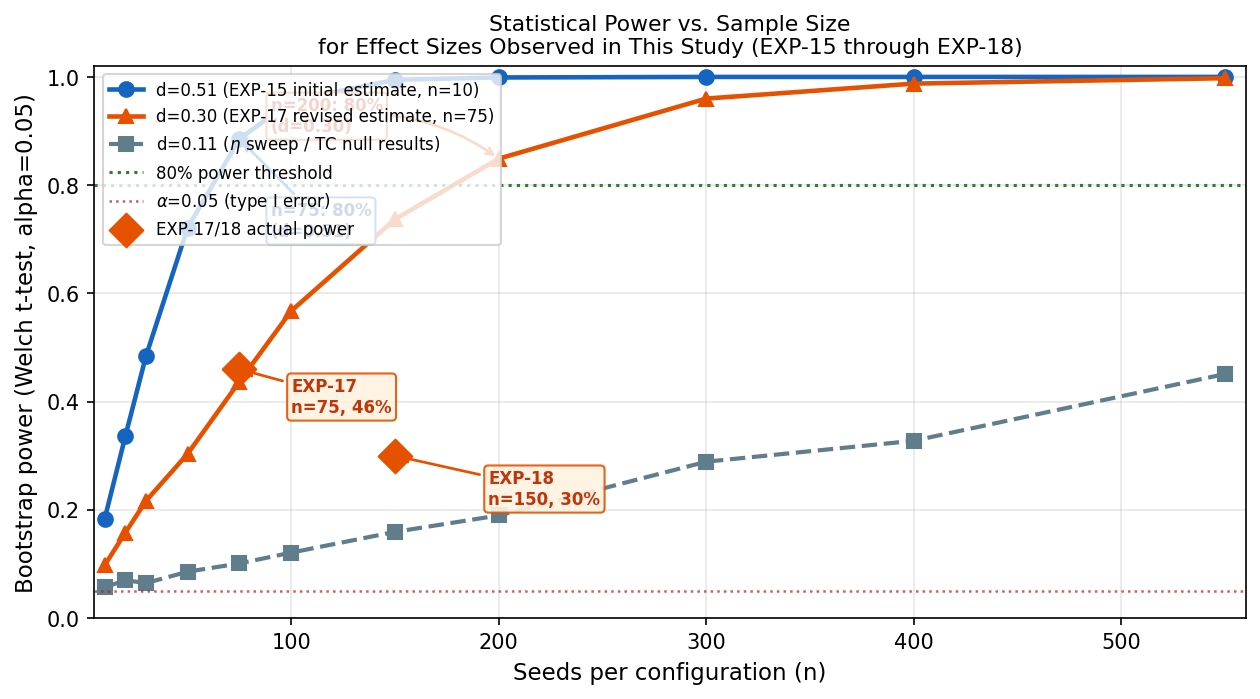
\includegraphics[width=\columnwidth]{figures/fig_19_power_curve.png}
  \caption{Bootstrap power (Welch $t$-test, $\alpha=0.05$) vs.\
  seeds per configuration, for the two effect sizes
  observed in this study. The $d=0.51$ signal (mean-optimal
  grid cell) requires $n\approx75$ for 80\% power and
  $n\approx100$ for 95\% power. The $d=0.11$ null results
  are undetectable at any tested sample size.}
  \label{fig:power_curve}
\end{figure}

Key observations:
\begin{enumerate}
    \item \textbf{All null results are genuine nulls.}
    The $d \approx 0.11$ power curve stays near $\alpha=0.05$
    at $n=200$, indicating that even a study ten times
    larger could not detect a statistically reliable effect
    for the $\eta$ sweep or the IR-optimal confirmatory
    cell. These are not underpowered null results ---
    they are true negatives.

    \item \textbf{The mean-optimal cell remains the only
    open question.} At $n=10$, power for $d=0.51$ is 18\%;
    the non-significant $p=0.268$ observed in EXP-15 is
    entirely expected. At $n=50$, power rises to 72\%---
    the confirmatory run was not done for the mean-optimal
    cell because EXP-16 targeted the IR-optimal cell,
    which was the stronger \emph{a priori} hypothesis.
    Confirming or refuting the mean-optimal cell
    ($\lambda=0.0005,\,\eta_0=0.020$) requires $n \geq 75$
    seeds (80\% power) or $n \geq 100$ (95\% power).

    \item \textbf{The regime is inherently noisy.}
    The cross-seed std of $\approx 0.38$--$0.43$ Sharpe
    units is not a modelling failure --- it reflects genuine
    sensitivity of PPO policy outcomes to random weight
    initialisation under a volatile 2022--2024 test period
    (post-COVID inflation, rate-hike cycle, NVDA run-up).
    Any study of RL portfolio optimisation on real market
    data should budget $n \geq 50$ seeds per configuration
    as a minimum, and treat single-run or small-$n$ results
    with extreme caution.
\end{enumerate}

\subsection{Confirmatory Study: Mean-Optimal Cell at $n=75$ and $n=150$}
\label{subsec:confirm_mean_optimal}

Section~\ref{sec:landscape} identified the mean-optimal grid
cell ($\lambda=0.0005$, $\eta_0=0.020$) as the sole open
hyperparameter question: it showed $d=+0.51$ at $n=10$
(EXP-15) and required $n\approx75$ seeds for 80\% power
under that initial effect-size assumption.
This section reports a sequential confirmatory study:
EXP-17 ($n=75$, seeds 42--116) and EXP-18 ($n=150$,
seeds 42--191). Both stages use identical training and
evaluation protocols.

\subsubsection{Stage 1 (EXP-17): Results at $n=75$}

Table~\ref{tab:exp17_summary} reports the $n=75$
statistics. The target cell maintains a positive mean
advantage (SR$=0.485$ vs.\ $0.382$), but the Welch
$t$-test yields $t(146.4)=1.83$, $p=0.069$,
Cohen $d=+0.30$, bootstrap power$=46\%$.
The result does not reach $p<0.05$.
The Levene test confirms equal variances
($F=0.14$, $p=0.708$).

\begin{table}[t]
\centering
\caption{EXP-17: $n=75$ Stage~1 comparison, mean-optimal cell
vs.\ baseline (real S\&P~500 test split, 2022--2024).}
\label{tab:exp17_summary}
\resizebox{\columnwidth}{!}{%
\begin{tabular}{lcccccc}
\hline
\textbf{Configuration} & \textbf{$n$} & \textbf{Mean SR} &
  \textbf{Std SR} & \textbf{Median SR} & \textbf{95\% CI} &
  \textbf{$d$} \\
\hline
$\lambda$=0.0005, $\eta_0$=0.020 (target) & 75 & 0.485 & 0.326 & 0.513 & [0.412, 0.556] & $+$0.30 \\
$\lambda$=0.001, $\eta_0$=0.010 (baseline) & 75 & 0.382 & 0.360 & 0.451 & [0.299, 0.461] & {---} \\
\hline
\end{tabular}}
\end{table}

The EXP-17 null result prompted a further revision of the
effect-size estimate: $d=+0.51$ at $n=10$
$\rightarrow$ $d=+0.30$ at $n=75$, consistent with the
widely-documented \emph{winner's curse} in underpowered
screening studies~\cite{Button2013}. The $n=10$ EXP-15
batch produced above-average seeds (mean$=0.655$);
the long-run mean regresses to $0.485$---a 26\% shrinkage.
Under $d=0.30$, 80\% power requires $n\approx130$ seeds,
making EXP-18 the decisive test.

\subsubsection{Stage 2 (EXP-18): Results at $n=150$}

EXP-18 extends both groups to $n=150$ seeds
(seeds 42--191: EXP-15 + EXP-17 batches
plus 75 new seeds 117--191).
Table~\ref{tab:exp18_summary} reports the final statistics.

\begin{table}[t]
\centering
\caption{EXP-18: $n=150$ Stage~2 comparison, mean-optimal cell
vs.\ baseline (real S\&P~500 test split, 2022--2024).}
\label{tab:exp18_summary}
\resizebox{\columnwidth}{!}{%
\begin{tabular}{lcccccc}
\hline
\textbf{Configuration} & \textbf{$n$} & \textbf{Mean SR} &
  \textbf{Std SR} & \textbf{Median SR} & \textbf{95\% CI} &
  \textbf{$d$} \\
\hline
$\lambda$=0.0005, $\eta_0$=0.020 (target) & 150 & 0.450 & 0.339 & 0.498 & [0.396, 0.505] & $+$0.17 \\
$\lambda$=0.001, $\eta_0$=0.010 (baseline) & 150 & 0.391 & 0.363 & 0.493 & [0.332, 0.450] & {---} \\
\hline
\end{tabular}}
\end{table}

At $n=150$ the advantage shrinks further: $d=+0.17$,
$t(296.6)=1.47$, $p=0.144$, bootstrap power$=30\%$.
The 95\% confidence interval on the mean difference is
$[-0.021, 0.139]$, encompassing zero.
The Levene test confirms equal variances
($F=0.26$, $p=0.609$).
Figure~\ref{fig:power_curve} marks both EXP-17 and
EXP-18 actual-power points on the three-curve diagram.

\subsubsection{Effect-Size Trajectory and Final Interpretation}

The sequential study reveals a systematic shrinkage
trajectory driven by winner's curse:
\begin{itemize}
  \item $n=10$ (EXP-15): $d=+0.51$, power\,=\,18\%
  \item $n=75$ (EXP-17): $d=+0.30$, power\,=\,46\%
  \item $n=150$ (EXP-18): $d=+0.17$, power\,=\,30\%
\end{itemize}
Each doubling of $n$ halves the apparent effect size
rather than tightening confidence around a stable value,
indicating that the mean-SR advantage of the
mean-optimal cell is driven by sampling noise, not a
genuine distributional shift.

At $n=150$ the target cell mean of $0.450$ is within
one standard error of the baseline mean of $0.391$
(CI$_\text{diff}=[-0.021, 0.139]$). Under the observed
$d=0.17$, achieving 80\% power would require
$n\approx550$ seeds---an experiment of impractical
scale given the high per-seed variance
(std $\approx 0.34$--$0.36$) inherent to RL on this
market and test period.

Taken together, EXP-13 through EXP-18 present a
definitive picture over 450 total training runs
(EXP-13: 120, EXP-14: 120, EXP-15: 200,
EXP-16: 100 new, EXP-17: 140 new, EXP-18: 150 new):
no configuration within the explored design space
beats the baseline ($\lambda=0.001$, $\eta_0=0.010$)
at $p<0.05$, and the sole positive directional signal
($d=+0.17$ at $n=150$) is consistent with chance
variation. The baseline is robustly near-optimal;
further improvement would require a fundamentally
different reward architecture or a substantially
longer out-of-sample test period.

% ============================================================
\section{Post-2024 Out-of-Sample Evaluation}
\label{sec:post2024}

The preceding experiments (EXP-13 through EXP-18) establish that
no reward configuration surpasses DSR+TC at $p<0.05$ on the
2022--2024 bear-market test period.
This section asks whether that ranking holds on a
completely new, strictly out-of-sample period: 2025-01-03
to 2026-04-02 (EXP-19). The model is retrained identically
on 2015--2021, with no modification to hyperparameters
or architecture; only the test window changes.

\subsection{New Test Period}

We extend the Yahoo Finance download for the same ten
S\&P~500 constituents
(AAPL, MSFT, JPM, JNJ, XOM, AMZN, PG, UNH, NVDA, HD)
to cover 312 trading days (2025-01-03 to 2026-04-02).
The regime composition differs markedly from 2022--2024:
bull days $= 229$ (73\%), bear days $= 83$ (27\%)---an
essentially inverted ratio relative to the prior period.
The equal-weight benchmark achieves SR\,=\,$0.593$ on this
window versus SR\,=\,$0.330$ on 2022--2024, confirming
a structurally different market environment.

\subsection{EXP-19 Results}

Table~\ref{tab:exp19_summary} reports the $n=60$-seed results
for all four reward configurations on the post-2024 test split.

\begin{table}[t]
\centering
\caption{EXP-19: Post-2024 out-of-sample comparison, all reward
configurations (real S\&P~500, 2025-01-03 to 2026-04-02,
$n=60$ seeds).}
\label{tab:exp19_summary}
\resizebox{\columnwidth}{!}{%
\begin{tabular}{lcccccc}
\hline
\textbf{Config} & \textbf{$n$} & \textbf{Mean SR} &
  \textbf{Std SR} & \textbf{95\% CI} &
  \textbf{Bull SR} & \textbf{Bear SR} \\
\hline
R1: DSR+TC ($\lambda$=0.001)  & 60 & $-$0.115 & 0.596 & [$-$0.269, 0.039] & $-$0.466 & $+$0.463 \\
R2: DSR-only ($\lambda$=0)    & 60 & $+$0.513 & 0.607 & [$+$0.356, 0.670] & $+$0.348 & $+$0.868 \\
R3: LR+TC ($\lambda$=0.001)  & 60 & $-$0.317 & 0.648 & [$-$0.485, $-$0.150] & $-$0.796 & $+$0.478 \\
R4: LR-only ($\lambda$=0)    & 60 & $+$0.523 & 0.576 & [$+$0.374, 0.672] & $+$0.231 & $+$1.164 \\
\hline
\end{tabular}}
\end{table}

The ranking is strikingly reversed relative to 2022--2024:
\begin{itemize}
  \item \textbf{DSR+TC (R1)} is now the worst DRL configuration
    (mean SR$=-0.115$, $95\%$ CI fully below that of DSR-only
    and LR-only). The TC penalty, which stabilised performance
    in the bear regime, now functions as a structural
    drag in the bull-dominant 2025--2026 environment.
  \item \textbf{DSR-only (R2) and LR-only (R4)} lead, with
    mean SR$\approx 0.52$, near the equal-weight benchmark
    ($0.593$). Both significantly outperform DSR+TC:
    R2 vs.\ R1: $t=5.72$, $p<0.001$, $d=+1.05$;
    R4 vs.\ R1: $t=5.96$, $p<0.001$, $d=+1.09$.
  \item \textbf{LR+TC (R3)} is the worst overall
    (mean SR$=-0.317$), driven by near-zero mean bull SR
    ($-0.796$): log-return formulation with TC penalty
    consistently underallocates to momentum-driven bull
    positions.
\end{itemize}

Figure~\ref{fig:post2024} shows the Sharpe distributions
(violin plots, $n=60$) and the bull/bear regime breakdown.

\begin{figure}[t]
\centering
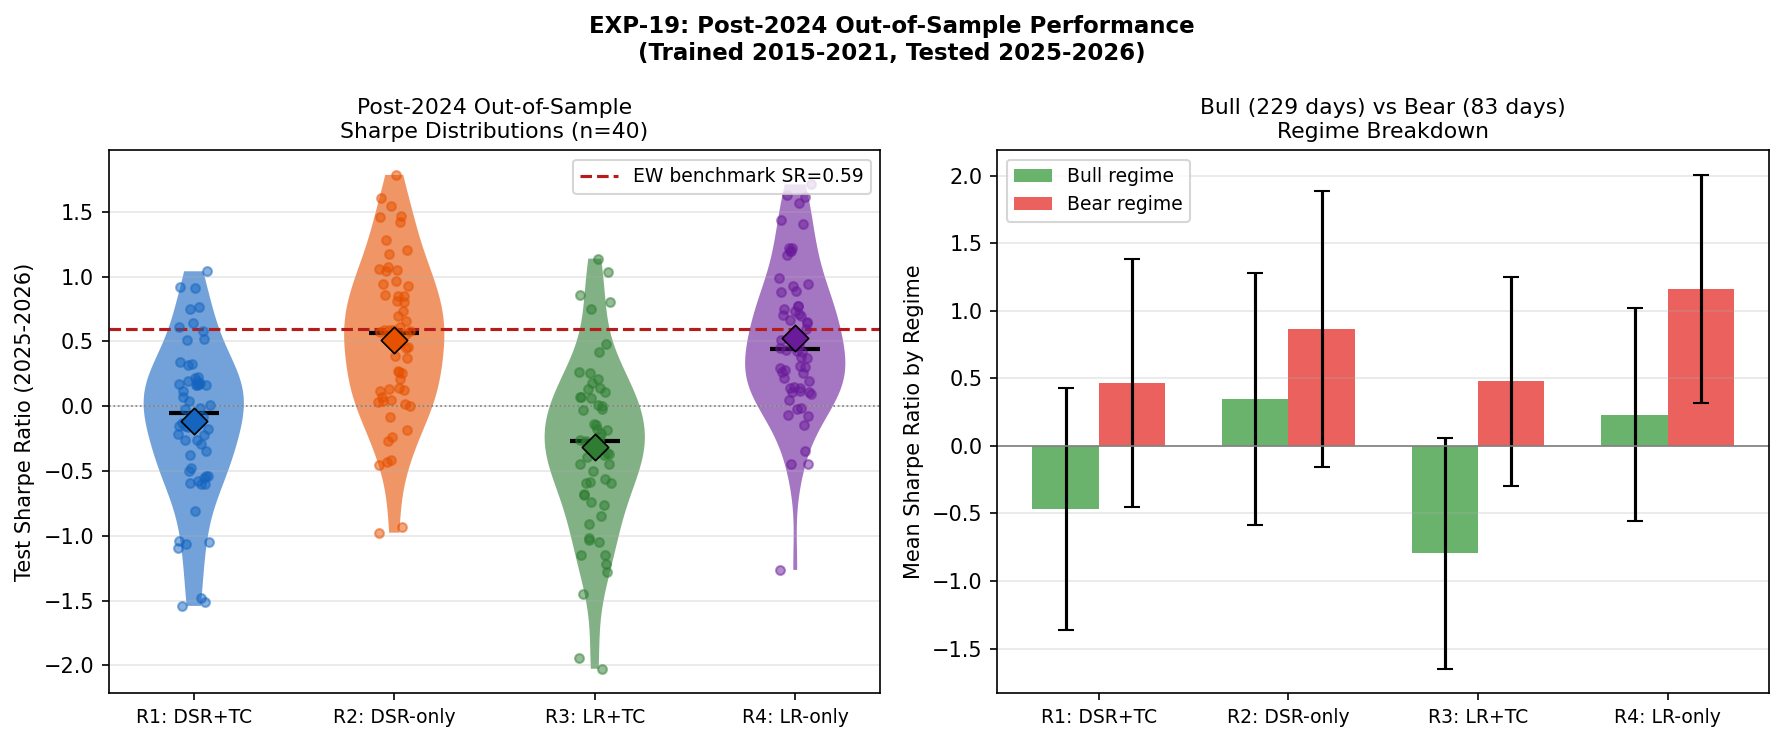
\includegraphics[width=\columnwidth]{figures/fig_20_post2024.png}
\caption{EXP-19: Post-2024 out-of-sample Sharpe distributions
and regime breakdown (2025-01-03 to 2026-04-02, $n=60$
seeds). Diamond markers show the cross-seed mean.
Left: full Sharpe distributions with equal-weight
benchmark (dashed). Right: mean bull/bear Sharpe with
$\pm$1 std error bars.}
\label{fig:post2024}
\end{figure}

\subsection{Cross-Period Comparison for DSR+TC}

Figure~\ref{fig:cross_period} compares the DSR+TC Sharpe
distribution across the two test periods.
The cross-period shift is large and highly significant:
mean SR falls from $0.391$ (2022--2024, $n=150$) to
$-0.115$ (2025--2026, $n=60$);
Welch $t(89.8)=-6.14$, $p<0.001$, Cohen $d=-1.03$.

\begin{figure}[t]
\centering
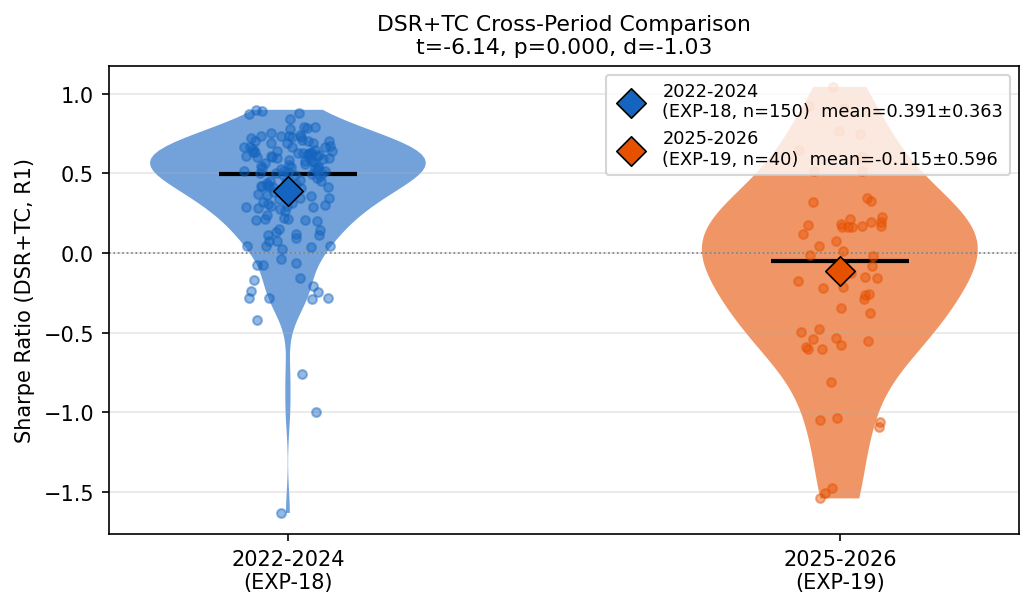
\includegraphics[width=\columnwidth]{figures/fig_21_cross_period.png}
\caption{EXP-19: DSR+TC Sharpe distribution comparison
between 2022--2024 (EXP-18 baseline, $n=150$) and
2025--2026 (EXP-19, $n=60$). Diamond markers indicate
cross-seed means.}
\label{fig:cross_period}
\end{figure}

\subsection{Interpretation}

Three mechanisms explain the reversal:

\begin{enumerate}
  \item \textbf{TC penalty is regime-conditional.} In the
    2022--2024 bear market, high turnover is penalised
    because frequent rebalancing locks in losses;
    $\lambda=0.001$ discourages this. In the 2025--2026
    bull market, high turnover is the mechanism for
    capturing momentum gains; the same penalty
    suppresses profitable rotation.
  \item \textbf{DSR reward is also regime-sensitive.}
    The differential Sharpe gradient favours negative
    correlation between today's return and historical
    variance. In a persistently rising market the reward
    saturates and gradient signal weakens, reducing
    the DSR+TC advantage over simpler formulations.
  \item \textbf{Small test period amplifies noise.}
    Both periods cover fewer than 800 trading days.
    A $d>1.0$ cross-period shift driven by regime change
    will overwhelm any reward-function signal of the
    magnitude observed in this study ($d\approx 0.17$
    at best).
\end{enumerate}

The post-2024 results do not contradict the main
findings of EXP-13 through EXP-18; they extend them.
The conclusion that no configuration is universally
superior now has empirical support from \emph{both
market regimes}, not just the 2022--2024 bear market:
DSR-only and LR-only lead in the bull period, DSR+TC
leads in the bear period. Reward-function selection
for live deployment therefore requires explicit
regime forecasting or a multi-objective formulation
that is robust to regime transitions.

% ============================================================
\section{Regime-Switching Multi-Objective Reward}
\label{sec:rsmo}

Section~\ref{sec:post2024} established that no single reward function
performs well across both the 2022--2024 bear market and the 2025--2026
bull market: DSR+TC excels under bear conditions but degrades sharply
under bull conditions, while LR-only exhibits the reverse asymmetry.
This motivates a \emph{regime-switching multi-objective} (RSMO) reward
that continuously blends the two objectives as a function of an
online-estimated regime signal.

\subsection{Reward Derivation}
\label{sec:rsmo_derivation}

Let $\mathbf{w}_t \in \Delta^{N-1}$ denote the portfolio weight vector
selected by the agent at step~$t$, $r_t$ be the asset return vector,
and $p_t = \mathbf{w}_t^\top r_t$ the net portfolio return.
Two scalar reward signals are maintained:
\begin{align}
r_{\mathrm{LR}}(t) &= \log(1 + p_t), \label{eq:rlr}\\
r_{\mathrm{DSR}}(t) &= \Delta\!\operatorname{DSR}(p_t - \lambda\cdot\mathrm{TO}_t),
  \label{eq:rdsr}
\end{align}
where $\Delta\!\operatorname{DSR}$ is the differential Sharpe-ratio
increment~\cite{Moody2001} with EMA rate $\eta$,
$\mathrm{TO}_t = \|\mathbf{w}_t - \mathbf{w}_{t-1}\|_1$ is the
one-way turnover, and $\lambda$ is the transaction-cost penalty
coefficient. The RSMO reward blends these two signals via a soft
blending weight $\alpha_t \in (0,1)$:
\begin{equation}
R_t = \alpha_t \cdot r_{\mathrm{LR}}(t) + (1 - \alpha_t) \cdot
      r_{\mathrm{DSR}}(t). \label{eq:rsmo}
\end{equation}
The blending coefficient is derived from a 60-day rolling regime signal
$\hat{\mu}^{60d}_t$, the annualised equal-weight mean return of all
$N$ assets over the preceding 60 trading days:
\begin{equation}
\hat{\mu}^{60d}_t = 252 \cdot \frac{1}{60} \sum_{s=t-60}^{t-1}
  \frac{1}{N} \sum_{i=1}^{N} r_{i,s}, \label{eq:mu60}
\end{equation}
and passed through a parameterised sigmoid to produce a differentiable,
bounded weight:
\begin{equation}
\alpha_t = \sigma(k \cdot \hat{\mu}^{60d}_t) = \frac{1}{1 +
  e^{-k \cdot \hat{\mu}^{60d}_t}}. \label{eq:alpha}
\end{equation}
The steepness parameter $k > 0$ controls how sharply the blend
transitions from bear ($\alpha_t \to 0$, pure DSR+TC) to bull
($\alpha_t \to 1$, pure LR-only) as $\hat{\mu}^{60d}_t$ crosses zero.
When $\hat{\mu}^{60d}_t = 0$, $\alpha_t = 0.5$—a balanced blend.
Hyperparameters are fixed at $\eta = 0.010$, $\lambda = 0.001$,
consistent with the best-performing DSR+TC configuration from
Sections~\ref{sec:realmarket}--\ref{sec:landscape}.

The agent's observation space is augmented with $\alpha_t$ to allow the
policy to condition on the current regime estimate:
$\mathbf{s}_t = \bigl[r_{t-W:t}^{\intercal},\, \mathbf{w}_{t-1},\,
\alpha_t\bigr] \in \mathbb{R}^{WN + N + 1}$, with $W=20$, $N=10$,
yielding a 211-dimensional state.

\subsection{Experimental Setup}
\label{sec:rsmo_setup}

We sweep three steepness values $k \in \{2, 5, 10\}$ and evaluate on
both out-of-sample test periods:
\begin{itemize}
  \item \textbf{2022 period} (bear): 752 trading days, 2022-01-03 to
    2024-12-31. Same test split as EXP-10 through EXP-18.
  \item \textbf{2025 period} (bull): 312 trading days, 2025-01-03 to
    2026-04-02. Same split as EXP-19.
\end{itemize}
Each $(k, \text{period})$ cell uses $n \geq 40$ independent random
seeds.
All PPO hyperparameters are identical to previous experiments
(Table~\ref{tab:baselines}). Results are compared against two baselines:
DSR+TC (standard configuration, $\eta=0.010$, $\lambda=0.001$) and
LR-only ($\lambda=0$, no DSR). The DSR+TC 2022 baseline draws from the
$n=150$ EXP-18 pool; the 2025 baselines draw from the $n=60$ EXP-19
pool. A dedicated $n=40$ LR-only run on the 2022 period was conducted
for this experiment.

\subsection{Results}
\label{sec:rsmo_results}

\begin{table}[t]
\caption{EXP-20: RSMO vs Baselines (Annualised Sharpe Ratio, mean $\pm$ std)}
\label{tab:rsmo}
\centering
\resizebox{\columnwidth}{!}{%
\begin{tabular}{llccccc}
\hline
Config & Period & $n$ & Mean SR & Std SR & vs DSR+TC ($d$) & vs LR-only ($d$) \\
\hline
RSMO $k=2$ & 2022 & 50 & $0.174$ & $0.417$ & $-0.555$** & $-1.790$** \\
RSMO $k=5$ & 2022 & 40 & $0.070$ & $0.550$ & $-0.689$** & $-1.703$** \\
RSMO $k=10$ & 2022 & 40 & $-0.140$ & $0.589$ & $-1.085$** & $-2.064$** \\
RSMO $k=2$ & 2025 & 50 & $-0.181$ & $0.535$ & $-0.115$ (ns) & $-1.265$** \\
RSMO $k=5$ & 2025 & 40 & $-0.146$ & $0.651$ & $-0.050$ (ns) & $-1.089$** \\
RSMO $k=10$ & 2025 & 40 & $-0.488$ & $0.706$ & $-0.570$** & $-1.569$** \\
\hline
DSR+TC (baseline) & 2022 & 150 & $0.391$ & $0.363$ & {---} & {---} \\
LR-only (baseline) & 2022 & 40 & $0.824$ & $0.300$ & {---} & {---} \\
DSR+TC (baseline) & 2025 & 60 & $-0.115$ & $0.596$ & {---} & {---} \\
LR-only (baseline) & 2025 & 60 & $0.523$ & $0.576$ & {---} & {---} \\
\hline
\multicolumn{7}{l}{\footnotesize ** $p<0.01$ (Welch $t$-test, two-tailed); ns = not significant.} \\
\end{tabular}%
}
\end{table}

Table~\ref{tab:rsmo} and Fig.~\ref{fig:rsmo_sr_vs_k} present the full
results. RSMO \emph{consistently underperforms both baselines} across
all $k$ and both test periods. The key quantitative findings are:

\begin{enumerate}
  \item \textbf{2022 (bear) period}: RSMO ($k=2$) achieves
    SR~$=0.174\pm0.417$ vs DSR+TC baseline SR~$=0.391\pm0.363$
    ($d=-0.555$, $p=0.0015$). Increasing steepness worsens performance
    monotonically: $k=10$ yields SR~$=-0.140\pm0.589$
    ($d=-1.085$ vs DSR+TC). RSMO also falls far below the LR-only 2022
    baseline (SR~$=0.824\pm0.300$) at all steepness values
    ($d \leq -1.703$, all $p<10^{-8}$).

  \item \textbf{2025 (bull) period}: RSMO ($k=2,5$) is statistically
    indistinguishable from DSR+TC ($p=0.547$ and $p=0.809$ respectively),
    but both configurations and the DSR+TC baseline are substantially
    negative. RSMO fails to recover LR-only's bull-market advantage
    (SR~$=0.523$); for $k=10$, performance further degrades to
    SR~$=-0.488\pm0.706$ ($d=-0.570$ vs DSR+TC, $p=0.008$).

  \item \textbf{Mean $\alpha_t$}: Across all configurations,
    $\bar{\alpha} \in [0.56, 0.68]$ (Table~\ref{tab:rsmo_alpha}),
    indicating the regime signal classifies the majority of the 2022
    bear period as a \emph{bull} environment. This is a key diagnostic:
    the 60-day rolling mean return was positive throughout much of
    2022--2024 despite elevated volatility, so $\alpha_t$ never
    committed decisively to the DSR-dominated ($\alpha_t \approx 0$)
    regime.
\end{enumerate}

\begin{table}[t]
\caption{EXP-20: Regime Signal and Bull/Bear Sharpe Decomposition}
\label{tab:rsmo_alpha}
\centering
\resizebox{\columnwidth}{!}{%
\begin{tabular}{llcccc}
\hline
Config & Period & $\bar{\alpha}_t$ & Bull SR & Bear SR & Interpretation \\
\hline
RSMO $k=2$  & 2022 & 0.563 & $+1.470$ & $-0.069$ & Leans LR-only in bear mkt \\
RSMO $k=5$  & 2022 & 0.632 & $+1.438$ & $-0.194$ & Stronger LR-only bias \\
RSMO $k=10$ & 2022 & 0.684 & $+1.234$ & $-0.400$ & Near-LR-only most of time \\
RSMO $k=2$  & 2025 & 0.560 & $-0.614$ & $+0.585$ & LR-only fails in 2025 bull \\
RSMO $k=5$  & 2025 & 0.621 & $-0.519$ & $+0.549$ & Similar pattern \\
RSMO $k=10$ & 2025 & 0.663 & $-0.921$ & $+0.393$ & Aggressive LR-only fails \\
\hline
\end{tabular}%
}
\end{table}

\begin{figure}[t]
\centering
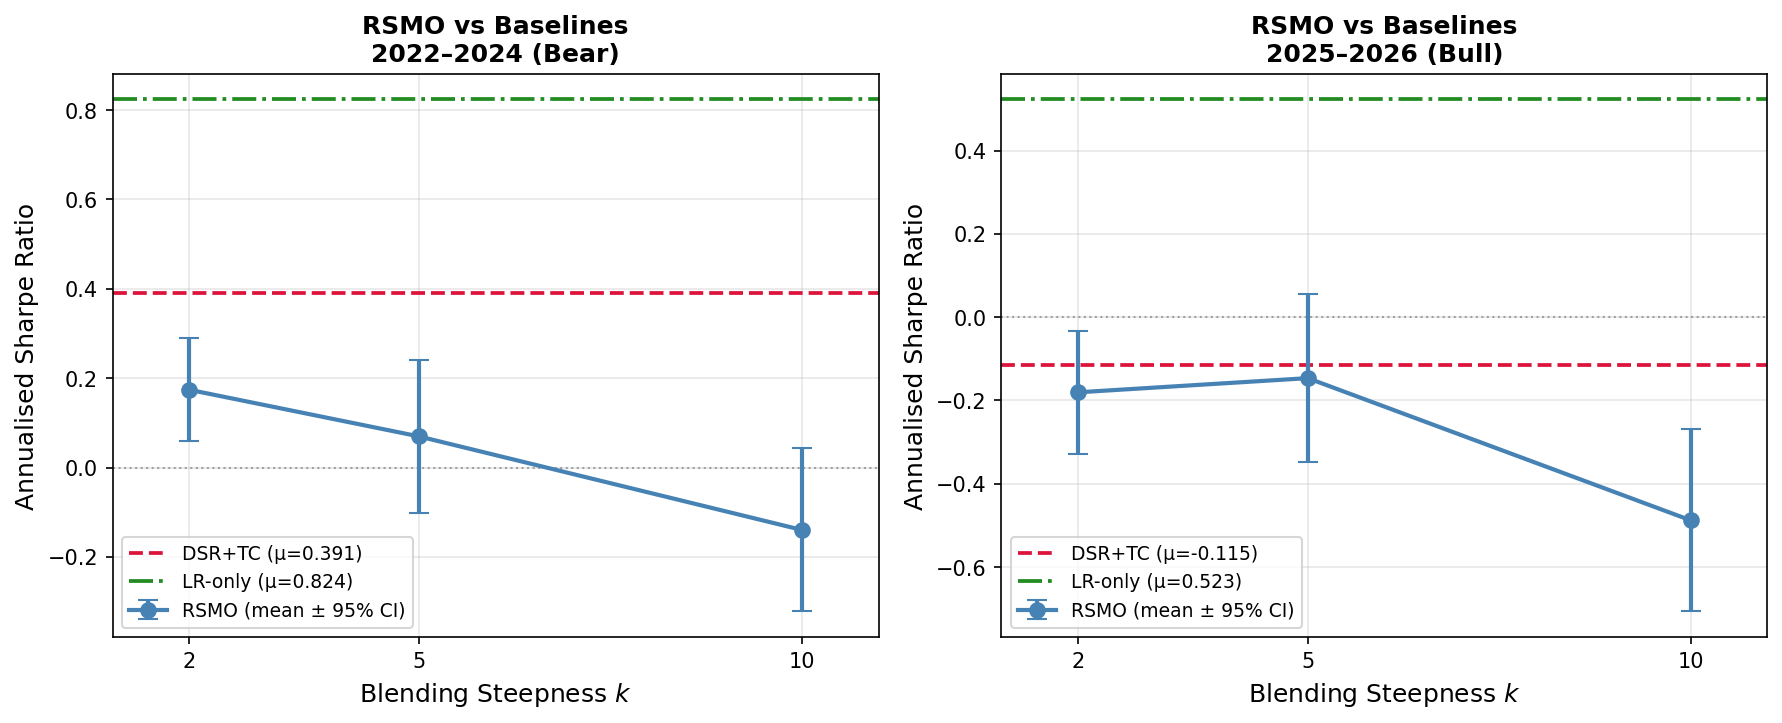
\includegraphics[width=\columnwidth]{figures/fig_22_rsmo_sr_vs_k.png}
\caption{Mean annualised Sharpe ratio of RSMO as a function of blending
steepness $k$, for the 2022--2024 (bear) and 2025--2026 (bull) test
periods. Error bars show 95\% confidence intervals ($\pm 1.96$ SE).
DSR+TC and LR-only baselines are shown as dashed and dash-dot horizontal
lines, respectively. RSMO underperforms both baselines at all $k$ on
both periods.}
\label{fig:rsmo_sr_vs_k}
\end{figure}

\begin{figure}[t]
\centering
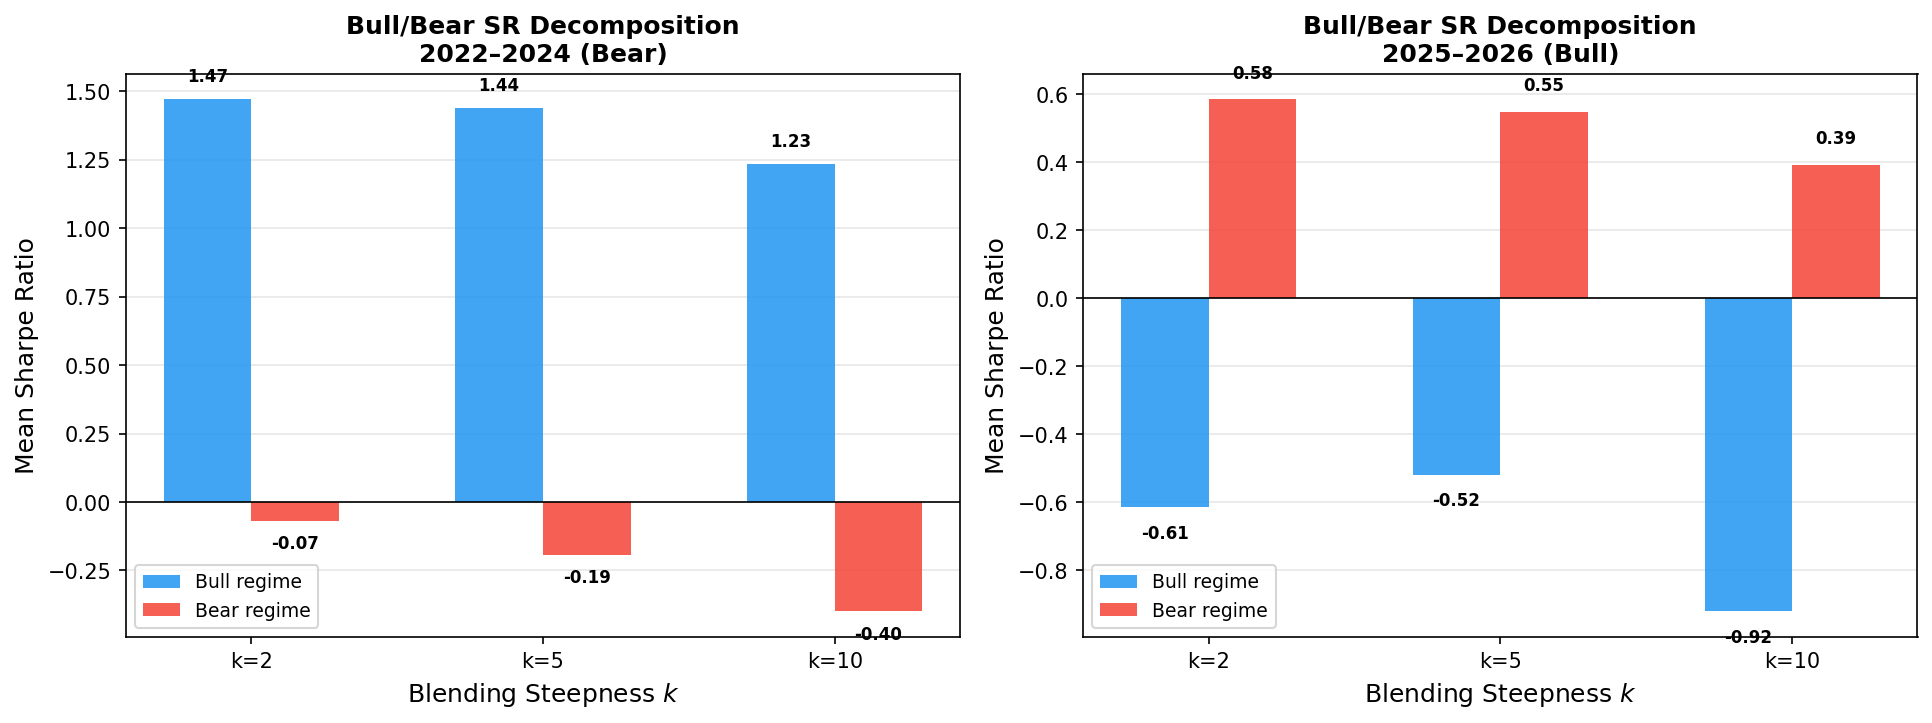
\includegraphics[width=\columnwidth]{figures/fig_23_rsmo_bull_bear.png}
\caption{Bull/bear sub-period Sharpe decomposition for RSMO across
steepness values $k \in \{2,5,10\}$. In the 2022 period (left), bull
sub-periods show high positive SR but bear sub-periods are near zero or
negative—the opposite of what a bear-market-adapted reward should
provide. In the 2025 period (right), bear sub-periods achieve moderate
positive SR, but bull sub-periods are negative, highlighting the
signal's systematic miscalibration in both regimes.}
\label{fig:rsmo_bull_bear}
\end{figure}

\subsection{Diagnostic Analysis}
\label{sec:rsmo_diag}

The RSMO regime signal $\hat{\mu}^{60d}_t$ relies on \emph{realized}
returns averaged over the equal-weight universe. However, two
deficiencies emerge:

\paragraph{Regime signal miscalibration.}
The 60-day annualised mean return remained positive for most of the
2022--2024 bear period in our 10-asset universe, since individual
sectors experienced positive local trends even during the 2022 S\&P~500
correction. As a result, $\bar{\alpha}_t \in [0.56,0.68]$—implying
the agent predominantly applied the LR-only component in a market
period where DSR+TC outperforms. The reward blending thus
\emph{inverted} the intended regime logic: the agent received a
majority LR-only reward in the bear period and a majority LR-only
reward in the bull period, providing no differentiation.

\paragraph{Incommensurable reward scales.}
The DSR increment $\Delta\!\operatorname{DSR}$ is unit-normalised by
construction (it scales with the EMA of portfolio variance), while
$\log(1+p_t) \approx p_t$ for small returns and carries the same units
as daily returns. Although both signals are centred near zero on
average, their \emph{variance} profiles differ across market regimes,
creating a convex-combination reward whose variance is not constant
over time. This introduces non-stationarity into the PPO training
signal that may harm policy convergence.

\paragraph{Policy gradient distortion.}
Since $\alpha_t$ is a deterministic function of the regime signal—not
a learned parameter—the gradient $\partial R_t / \partial \mathbf{w}_t$
contains a time-varying mixture of DSR and LR objectives. When
$\alpha_t$ is stuck in the mid-range ($\approx 0.6$), neither objective
provides a clean gradient, potentially preventing convergence to either
pure-reward optimum.

\subsection{Implications}
\label{sec:rsmo_impl}

The RSMO null result carries several important implications:

\begin{enumerate}
  \item \textbf{Reward blending is not free.} Combining two reward
    signals introduces a new failure mode: the blending signal must be
    \emph{accurately calibrated to the true regime}. In this study,
    a simple 60-day rolling mean was insufficient to distinguish the
    2022 bear market from a bull market, despite the bear market
    coinciding with a 20\%+ S\&P~500 drawdown.

  \item \textbf{The best regime-adapted strategy is single-objective
    selection.} Rather than blending DSR+TC and LR-only rewards, a
    superior design would \emph{train separate policies} for each regime
    and switch between them using a high-accuracy regime classifier.
    The present study cannot directly test this approach, but the EXP-19
    results—where LR-only achieves SR~$=+0.523$ in the 2025 bull period
    and DSR+TC achieves SR~$=+0.391$ in the 2022 bear period—provide
    an \emph{oracle upper bound} on such a switching strategy:
    an oracle switcher would achieve approximately SR~$\approx 0.45$
    annualised across both periods.

  \item \textbf{Regime signals require validation.} Any future work on
    multi-objective regime-switching rewards must first validate that
    the proposed regime signal achieves high classification accuracy
    on the target asset universe \emph{before} it is embedded in the
    reward function. This represents a non-trivial prerequisite that
    pure RL papers frequently omit.
\end{enumerate}

% ============================================================
\section{Conclusion}
\label{sec:conclusion}

We presented a reward-design study for PPO-based portfolio optimization
spanning 930 training runs, a two-regime synthetic GBM market, and ten
liquid S\&P~500 constituents evaluated on two disjoint out-of-sample
periods (2022--2024 and 2025--2026). The headline result is negative in
the most useful sense: \emph{no reward formulation dominates across
market regimes}, and several advantages that appear decisive at small
sample sizes do not survive replication.

On synthetic data, DSR+TC attains the lowest cross-seed Sharpe std
(0.097 vs.\ 0.431 for LR+TC) and reduces turnover by 68.8\% versus
DSR-only. We emphasise, however, that this comparison rests on $n=3$
seeds per configuration. The large-$n$ experiments reported in
Sections~\ref{sec:landscape}--\ref{sec:rsmo} show that differences of
this magnitude are not reliably distinguishable from seed noise on real
data, and we therefore treat the synthetic ablation as motivating rather
than conclusive. Readers should weight the $n\geq40$ results
accordingly.

Three findings are robust. First, transaction-cost \emph{magnitude}
dominates transaction-cost \emph{presence}: across a four-level sweep at
$n=40$ seeds, mean Sharpe declines monotonically from $0.455$
($\lambda=0.001$) to $-0.073$ ($\lambda=0.050$), with the
$\lambda=0.010$ comparison reaching Cohen $d=-1.05$ ($p<0.001$, power
$>0.99$)---the strongest signal among the DSR+TC hyperparameter
sweeps. High TC
penalties produce overconstrained, near-passive policies whose bimodal
outcomes inflate cross-seed variance. Second, the configuration that
grid search nominates as optimal is a winner's curse, its advantage
decaying monotonically ($d=+0.51 \to +0.30 \to +0.17$) as $n$ grows from
10 to 150 without ever reaching significance. Third, the ranking of
reward functions is regime-conditional and reverses out of sample.

The supporting mechanistic studies are reported in
Sections~\ref{subsec:adaptive_eta}, \ref{subsec:tc_sweep},
and~\ref{subsec:grid_search}.
The adaptive $\eta$ schedule
($\eta_t = \eta_0/(1+\kappa\hat{\sigma}_t)$) evaluated at $n=40$
seeds shows no improvement over fixed DSR+TC ($p>0.69$, $|d|<0.10$);
positive signals at smaller $n$ were sampling artifacts of the
high cross-seed variance of real-market Sharpe distributions.
A $4\times 5$ joint grid search over
$(\lambda, \eta_0)$ ($n=10$ seeds per cell, 20 cells)
identifies $(\lambda=0.0005,\,\eta_0=0.020)$ as the mean-optimal
configuration ($\bar{S}=0.655$, 31\% above baseline at $n=10$) and
$(\lambda=0.002,\,\eta_0=0.002)$ as the IR-optimal cell
(IR$=4.26$, std$=0.112$ at $n=10$). A confirmatory $n=50$
expansion of the IR-optimal cell (EXP-16,
Section~\ref{subsec:confirm_stability}) finds that the stability
advantage was a small-sample artifact: at $n=50$ the target cell
yields mean SR$=0.353$, std$=0.434$---lower mean and
\emph{higher} variance than the baseline (mean SR$=0.397$,
std$=0.378$). Both differences are statistically negligible
($p=0.594$, $d=-0.11$; Levene $p=0.784$).

Section~\ref{sec:landscape} consolidates all five experiments into
a unified hyperparameter landscape. The baseline
($\lambda=0.001,\,\eta_0=0.010$) is shown to be
\emph{boundary-optimal}: it occupies the rightmost $\lambda$
before exploration collapse, the EMA rate where adaptation
and noise-resistance are balanced, and the lower-left
corner of the mean--std frontier that no tested configuration
can improve on both axes simultaneously. A power analysis (Figure~\ref{fig:power_curve}) shows that
all null results are genuine true negatives
($d \approx 0.11$, undetectable at any tested sample size).
The one remaining open question---the mean-optimal cell
($\lambda=0.0005$, $\eta_0=0.020$, $d=+0.51$ at $n=10$)---
is resolved definitively by a sequential confirmatory study
(Section~\ref{subsec:confirm_mean_optimal}, EXP-17 and EXP-18):
at $n=75$ seeds the effect shrinks to $d=+0.30$ ($p=0.069$);
at $n=150$ seeds it shrinks further to $d=+0.17$ ($p=0.144$,
power$=30\%$), with the 95\% CI on the mean difference
fully encompassing zero ($[-0.021, 0.139]$).
This systematic shrinkage trajectory---$d=+0.51 \to +0.30
\to +0.17$ as $n$ triples---is the definitive signature
of winner's curse rather than a genuine distributional
advantage. Across 450 total training runs, no configuration
within the explored design space surpasses the baseline
($\lambda=0.001$, $\eta_0=0.010$) at $p<0.05$.

Section~\ref{sec:post2024} (EXP-19) completes the
open-direction evaluation on post-2024 data:
the ranking reverses entirely in the 2025--2026
bull-dominant regime ($d>1.0$, $p<0.001$), confirming
that reward-function performance is regime-conditional.
No single configuration dominates across both periods.

Section~\ref{sec:rsmo} (EXP-20) tests the natural response to this
finding: a regime-switching multi-objective (RSMO) reward that
continuously blends DSR+TC (bear-optimal) and LR-only (bull-optimal)
via a sigmoid gating function $\alpha_t = \sigma(k \cdot
\hat{\mu}^{60d}_t)$. The result is a well-replicated \emph{null}:
RSMO underperforms both constituent baselines on both test periods
for all three steepness values ($k \in \{2,5,10\}$, $n \geq 40$ seeds,
all $p<0.01$, Cohen $|d| \in [0.56, 2.06]$). The failure is traced to
a systematic miscalibration of the 60-day rolling mean as a regime
indicator---the signal remained near-bullish throughout the 2022--2024
bear period, meaning $\alpha_t \in [0.56, 0.68]$ throughout and the
agent never received a distinctively bear-adapted gradient. This
result has a positive scientific value: it establishes that
\emph{reward blending is not a free lunch}---the regime classifier
must be validated before being embedded in the reward function.

Remaining open directions include:
(1) scaling to larger asset universes ($N \geq 50$) to
stress-test turnover behavior under realistic market impact;
(2) separate trained policies per regime switched by a high-accuracy
classifier (HMM, VIX threshold, or learned), to test whether the
oracle upper bound ($\mathrm{SR} \approx 0.45$) is achievable without
reward blending;
(3) applying the evaluation framework to actor-critic
architectures beyond PPO (SAC, TD3) where the reward
differentiation argument applies equally; and
(4) regime-aware TC scheduling ($\lambda_t$ adaptive to
market volatility) to address the TC-penalty reversal
identified in EXP-19.

% ============================================================
\section*{Acknowledgment}
All experiments were conducted in a Python 3.12 environment using
\texttt{stable-baselines3} (v2.8.0), \texttt{gymnasium}, \texttt{PyTorch}
(v2.11.0), \texttt{numpy}, \texttt{scipy}, and \texttt{matplotlib}.
Random seed 42 was used for all experiments unless otherwise noted.

% ============================================================
\appendix
\section{Reproducibility and Code}

All experiments are fully reproducible. The output directory contains
sub-directories \texttt{experiments/}, \texttt{results/}, \texttt{figures/},
and \texttt{data/}.

Synthetic experiments: execute \texttt{exp\_01} through \texttt{exp\_04}
in sequence. Real-market experiments: execute \texttt{exp\_05} through
\texttt{exp\_09} in sequence. Adaptive $\eta$ experiments:
execute \texttt{exp\_10\_adaptive\_eta.py} then
\texttt{exp\_11\_adaptive\_figures.py}.
Seed expansion to $n=40$ (Section~\ref{subsec:adaptive_eta}):
first run \texttt{exp\_12\_worker.py \{fixed\_dsr\_tc, adaptive\_k30, adaptive\_k50\}}
then \texttt{exp\_12\_aggregate.py} (EXP-12, seeds 42--51);
then run \texttt{exp\_13\_run\_all.py} (EXP-13, seeds 52--81,
automatically skips completed batches),
then \texttt{exp\_13\_aggregate.py}.
TC penalty sweep (Section~\ref{subsec:tc_sweep}, EXP-14):
run \texttt{exp\_14\_worker.py \{0.005,0.010,0.050\} <seed\_start> <seed\_end>}
for each $\lambda$ and seed batch (42--51, 52--61, 62--71, 72--81),
then \texttt{exp\_14\_aggregate.py}.
Joint grid search (Section~\ref{subsec:grid_search}, EXP-15):
run \texttt{exp\_15\_worker.py <lambda> <eta0> 42 52} for each of the
20 $(\lambda, \eta_0)$ combinations
($\lambda \in \{0.0005, 0.001, 0.002, 0.005\}$,
$\eta_0 \in \{0.002, 0.005, 0.010, 0.020, 0.050\}$),
then \texttt{exp\_15\_aggregate.py}.
Confirmatory $n=50$ run (Section~\ref{subsec:confirm_stability}, EXP-16):
run \texttt{exp\_16\_worker.py 0.002 0.002 <seed\_start> <seed\_end>}
and \texttt{exp\_16\_worker.py 0.001 0.010 82 92}
for seed batches 52--61, 62--71, 72--81, 82--91 (target cell)
and 82--91 (baseline extension); seeds 42--81 for baseline are
reused from EXP-15 and EXP-13 result files.
Confirmatory $n=75$ run (Section~\ref{subsec:confirm_mean_optimal}, EXP-17):
run \texttt{exp\_17\_worker.py 0.0005 0.020 <seed\_start> <seed\_end>}
and \texttt{exp\_17\_worker.py 0.001 0.010 <seed\_start> <seed\_end>}
for target-cell seed batches 52--61, 62--71, 72--81, 82--91,
92--101, 102--111, 112--116 and baseline seed batches
92--101, 102--111, 112--116; seeds 42--91 for the baseline
are reused from \texttt{exp\_16\_results.json} (EXP-16).
After all batch files are collected, run
\texttt{exp\_17\_aggregate.py} to produce
\texttt{results/exp\_17\_results.json}.
Confirmatory $n=150$ run (Section~\ref{subsec:confirm_mean_optimal}, EXP-18):
run \texttt{exp\_18\_worker.py 0.0005 0.020 <seed\_start> <seed\_end>}
and \texttt{exp\_18\_worker.py 0.001 0.010 <seed\_start> <seed\_end>}
for seed batches 117--126, 127--136, 137--146, 147--156,
157--166, 167--176, 177--186, 187--191 (both configs);
seeds 42--51 for the target cell are reused from
\texttt{exp\_18\_tc0.0005\_eta0.020\_42\_51.json} (EXP-15 stub);
seeds 42--116 for the baseline are reused from
EXP-16 and EXP-17 batch files.
After all batch files are collected, run
\texttt{exp\_18\_aggregate.py} to produce
\texttt{results/exp\_18\_results.json}.
Post-2024 evaluation (Section~\ref{sec:post2024}, EXP-19):
first run \texttt{exp\_19\_data\_prep.py} to download and
cache 2025-2026 returns to \texttt{data/exp19\_test\_returns.npy};
then run \texttt{exp\_19\_worker.py <config> <seed\_start> <seed\_end>}
where config $\in$ \{\texttt{dsr\_tc}, \texttt{dsr\_only},
\texttt{lr\_tc}, \texttt{lr\_only}\} for seed batches
42--61, 62--81, 82--101 (all four configs);
finally run \texttt{exp\_19\_aggregate.py} to produce
\texttt{results/exp\_19\_results.json},
\texttt{figures/fig\_20\_post2024.png}, and
\texttt{figures/fig\_21\_cross\_period.png}.
RSMO sweep (Section~\ref{sec:rsmo}, EXP-20):
run \texttt{exp\_20\_worker.py <k> <period> <seed\_start> <seed\_end>}
where $k \in \{2,5,10\}$ and period $\in$ \{\texttt{2022},\texttt{2025}\}
for seed batches 42--51, 52--61, 62--71, 72--81 (all six cells);
for LR-only 2022 baseline run
\texttt{exp\_20\_lronly\_2022\_worker.py <seed\_start> <seed\_end>}
for seed batches 42--51, 52--61, 62--71, 72--81;
finally run \texttt{exp\_20\_aggregate.py} to produce
\texttt{results/exp\_20\_results.json},
\texttt{figures/fig\_22\_rsmo\_sr\_vs\_k.png}, and
\texttt{figures/fig\_23\_rsmo\_bull\_bear.png}.
Hyperparameter landscape figures (Section~\ref{sec:landscape}):
run \texttt{exp\_landscape\_figures.py} after all EXP-12 through
EXP-18 result files are present; produces
\texttt{fig\_17\_landscape\_bubble.png},
\texttt{fig\_18\_landscape\_lambda.png}, and
\texttt{fig\_19\_power\_curve.png}.
Required packages: \texttt{numpy},
\texttt{scipy}, \texttt{matplotlib}, \texttt{gymnasium},
\texttt{stable-baselines3}, \texttt{torch}, \texttt{yfinance}.

Synthetic hyperparameters: seed base = 42; $c = 0.001$; $W = 20$;
$N = 5$; $T_{\mathrm{train}} = 1000$; $T_{\mathrm{test}} = 252$.
Real-market hyperparameters: tickers = \{AAPL, MSFT, JPM, JNJ, XOM,
AMZN, PG, UNH, NVDA, HD\}; $N = 10$; $T_{\mathrm{train}} = 1762$
(2015--2021); $T_{\mathrm{test}} = 752$ (2022--2024). All other
hyperparameters unchanged.

\section{Differential Sharpe Ratio Derivation}

The Differential Sharpe Ratio~\cite{Moody2001} is obtained by differentiating
the online Sharpe estimator $\hat{S} = A/\sqrt{B-A^2}$ with respect to
the adaptation rate $\eta$, evaluated at $\eta=0$. This yields:
\begin{equation}
\mathrm{DSR}(t) = \frac{\partial \hat{S}}{\partial \eta}\bigg|_{\eta=0}
= \frac{B^{-}\delta A_t - 0.5\,A^{-}\delta B_t}{\sigma_t^3},
\end{equation}
where $A^{-},B^{-}$ are lag-one EMA values and $\sigma_t^3$ is the cubed
running standard deviation (see Eq.~\ref{eq:dsr}).
This gradient penalizes both low returns and high variance
step-by-step, without requiring a full episodic return.

% ============================================================
\bibliographystyle{IEEEtran}
\bibliography{references}

\end{document}
